\documentclass[11pt]{book}
\usepackage{amssymb}
\usepackage{amsmath}
\usepackage{amsthm}
\usepackage{fullpage}
\usepackage{hyperref}
\usepackage{multicol}
\usepackage{svg}
\usepackage[h]{esvect}
\usepackage{graphicx}
\usepackage{gensymb}
\setlength{\parskip}{1ex}
\setlength{\parindent}{0pt}
\def\N {{\mathbb N}}
\def\Z {{\mathbb Z}}
\def\R {{\mathbb R}}
\def\comp {{\mathrm{comp}}}
\def\proj {{\mathrm{proj}}}
\def\Grad {\mathrm{grad\,}}
\def\Div {\mathrm{div\,}}
\def\Curl {\mathrm{curl\,}}

\newcommand{\partialderiv}[2] {\frac{\partial #1}{\partial #2}}
\newcommand{\Implies}{\mbox{ IMPLIES }}
\newcommand{\Or}{\mbox{ OR }}
\renewcommand{\And}{\mbox{ AND }}
\newcommand{\Not}{\mbox{NOT}}
\newcommand{\Iff}{\mbox{ IFF }}
\newcommand{\True}{\mbox{T}}
\newcommand{\False}{\mbox{F}}
\newcommand{\norm}[1]{\lVert #1 \rVert}
\usepackage{listings}

\usepackage{tikz}
\usepackage{pgffor}
\usetikzlibrary{graphs,arrows.meta,trees,arrows}

\usepackage{xcolor}

\definecolor{codegreen}{HTML}{237e02}
\definecolor{codegray}{rgb}{0.5,0.5,0.5}
\definecolor{codepurple}{HTML}{8F4673}
\definecolor{codebrown}{HTML}{ce9178}
\definecolor{codecyan}{HTML}{098658}
\lstdefinestyle{pythonstyle}{
    commentstyle=\color{codegreen},
    keywordstyle=\color{codepurple},
    numberstyle=\tiny\color{codegray},
    stringstyle=\color{codebrown},
    basicstyle=\ttfamily\small,
    breakatwhitespace=false,         
    breaklines=true,                 
    captionpos=b,                    
    keepspaces=true,                 
    numbers=none,                    
    numbersep=5pt,                  
    showspaces=false,                
    showstringspaces=false,
    showtabs=false,                  
    tabsize=2
}

\lstset{style=pythonstyle}

\newtheorem{theorem}{Theorem}[section]
\newtheorem{corollary}{Corollary}[theorem]
\newtheorem{lemma}[theorem]{Lemma}
\newtheorem{definition}[theorem]{Definition}
\newcounter{example}[section]
\newenvironment{example}[1][]{\refstepcounter{example}\par\medskip
   \noindent \textbf{Example~\theexample. #1} \rmfamily}{\par \begin{flushright} \textbf{End of Example~\theexample} \end{flushright}}

\begin{document}

\title{Notes on Multivariable Calculus}
\author{Kevin Gao}
\maketitle

\chapter{Vectors}

\section{3D Coordinate Systems}

\subsection{3D Space}
Similar to the 2D coordinate system, we have the $x$ and $y$-axes. In addition, we add a new vertical $z$-axis. The direction of $z$-axis is determined by the right-hand rule. Such system is called the right-hand system.

\begin{figure}[h]
    \centering
    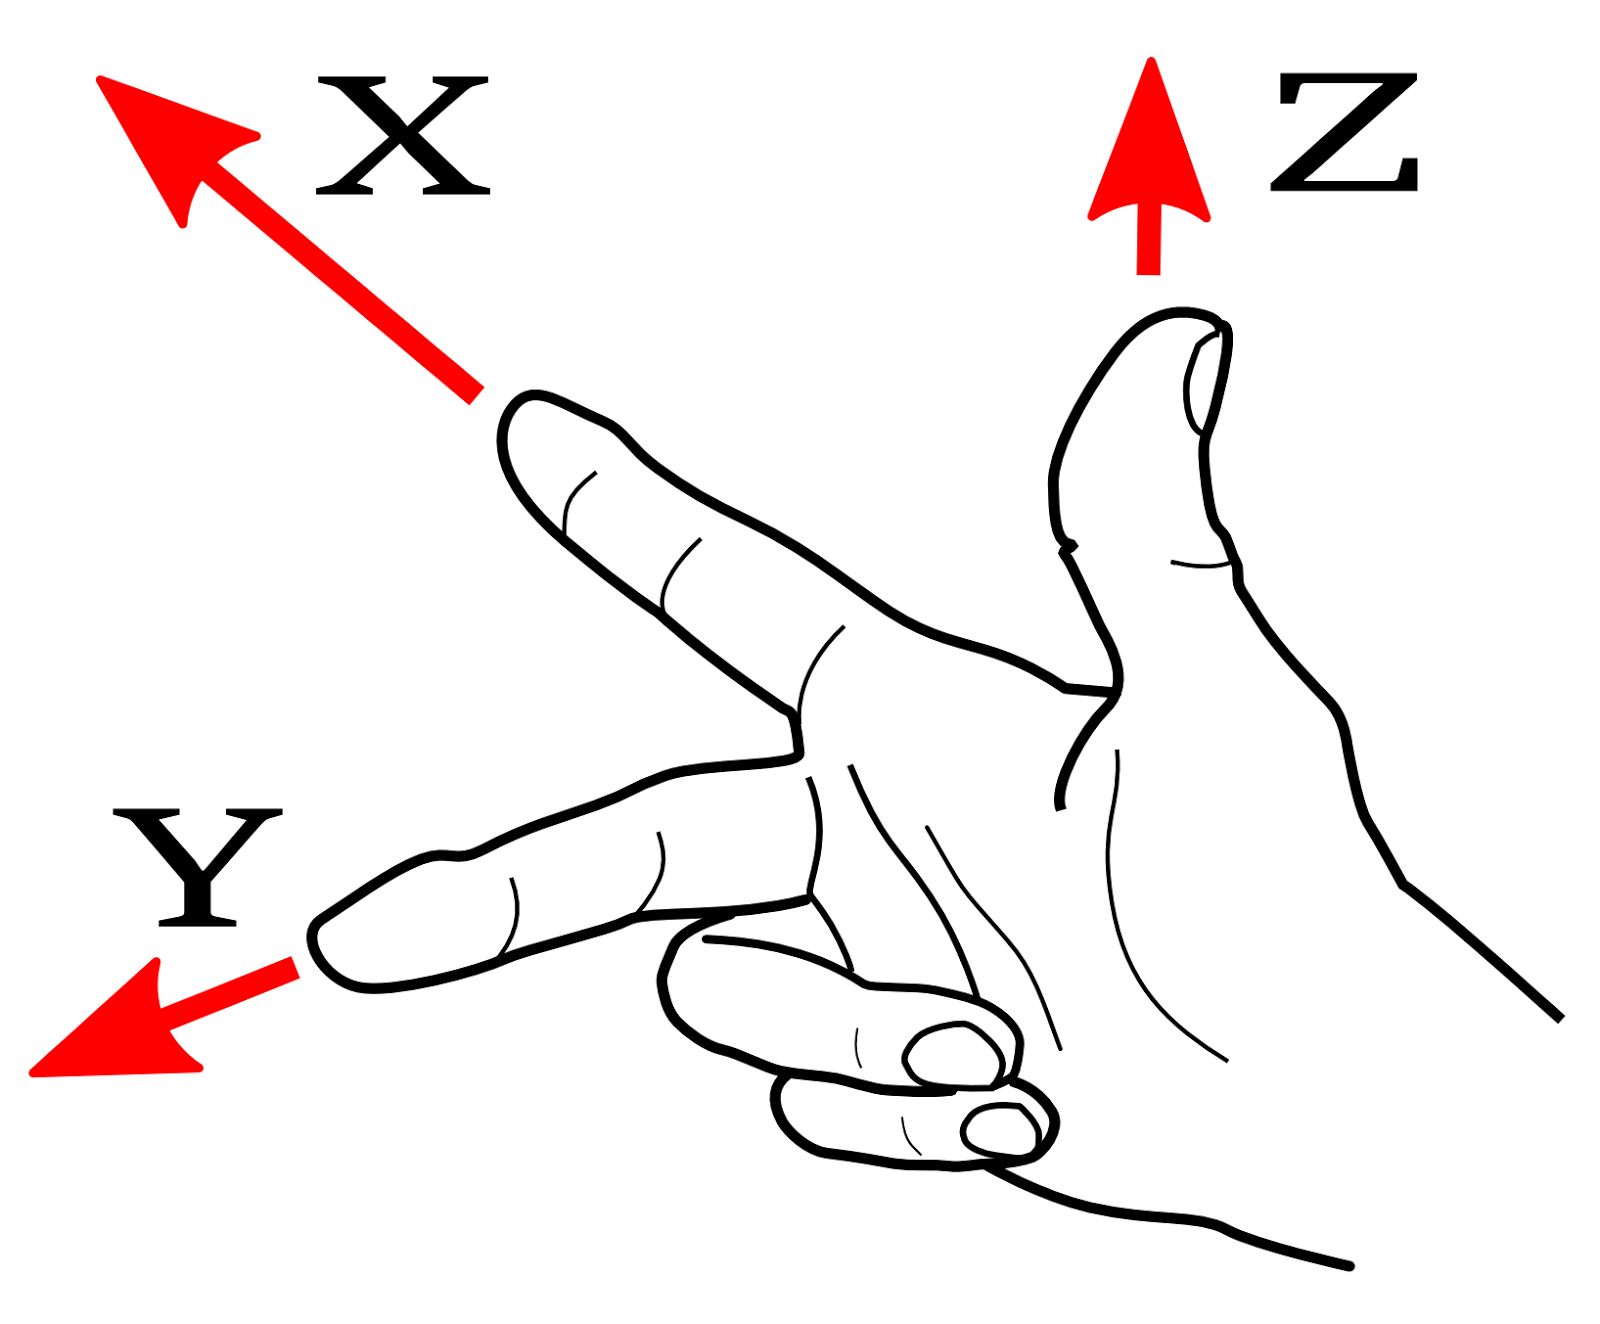
\includegraphics[width=0.3\textwidth]{figures/right-hand-rule.png}
    \caption{Right-hand rule}
\end{figure}
\hfill

In a right-hand system, the axes $x,y,z$ goes in clockwise, following ``index finger, middle finger, thumb''. The thumb pointing up is the $z$-axis. The origin $O$ is located at $(0,0,0)$.

Each two of the three axes form planes, giving us three planes: $xy,xz,yz$-planes.

We can project a point in the 3D coordinate onto the planes. For the point $P=(a,b,c)$, its projection onto $xy$-plane is $(a,b,0)$. Similarly, its projection onto $yz,xz$-planes are $(0,b,c)$ and $(a,0,c)$, respectively.

The Cartesian product $\R\times\R\times\R = \{(x,y,z) \mid x,y,z\in\R\}$ is the set of ordered triples of real numbers. It is denoted $\R^3$. These triples correspond to points in the three-dimensional coordinate.

\subsection{Surfaces and Solids}
Geometrically, equations involving $x,y,z$ represents a surface in $\R^3$. A 2D line is analogous to a plane in 3D, and a 2D circle is analogous to a cylinder in 3D.

\begin{example}
What surface in $\R^3$ is represented by each of the following equations? \\ (a) $z-3$ (b) $y-5$

(a) The equation $z-3$ represents the set $\{(x, y, z) \mid z - 3\}$, which is the set of all points in $\R^3$ whose z-coordinate is 3 ($x$ and $y$ can each be any value). This is the horizontal plane that is parallel to the $xy$-plane and three units above it.

(b) The equation $y-5$ represents the set of all points in $\R^3$ whose $y$-coordinate is 5. This is the vertical plane that is parallel to the $xz$-plane and five units to the right of it.
\end{example}

\subsection{Distance Formula}

The distance formula is similar to the distance formula in 2D.

\begin{theorem}[Distance formula in 3D]
The distance $|P_1P_2|$ between points $P_1=(x_1,y_1,z_1)$ and $P_2=(x_2,y_2,z_2)$.
$$
|P_1P_2| = \sqrt{(x_2-x_1)^2+(y_2-y_1)^2+(z_2-z_1)^2}
$$
\end{theorem}

The set of points that are equidistant to a point forms a sphere shell in 3D.

\begin{theorem}[Equation of sphere]
An equation of a sphere with center $C=(h,k,l)$ and radius $r$ is
$$
(x-h)^2+(y-k)^2+(z-l)^2 = r^2
$$
In particular, if the center is the origin, then an equation of the sphere is
$$
x^2+y^2+z^2 = r^2
$$
\end{theorem}

\section{Vectors}

\subsection{Definition}

Formally, we define vectors in the following way:

\begin{definition}[Vector Space]
A vector space is a field $(V,+,\cdot)$ where $V$ is a set of objects called vectors, together with a rule $+:\, V\times V\to V$ for adding $\alpha,\beta\in V$ to product $\alpha+\beta\in V$ and another rule $\cdot:\, V\times V\to V$ for multiplying vector $v\in V$ by any $k\in\R$ to produce $kv\in V$. In addition, the field must satisfy that

\begin{multicols}{2}
\begin{enumerate}
    \item $\alpha+\beta = \beta+\alpha$
    \item $(\alpha+\beta)+\gamma = \alpha+(\beta+\gamma)$
    \item $\alpha+0=\alpha$
    \item $\alpha+(-\alpha)=0$
    \item $k(\alpha+\beta)=k\alpha+k\beta$
    \item $(k+s)\alpha=k\alpha+s\alpha$
    \item $k(s\alpha)=(ks)\alpha$
    \item $1\alpha=\alpha$
\end{enumerate}
\end{multicols}
for the zero vector $0$, $s,k\in\R$, and $-\alpha \in V$ for all $\alpha \in V$.
\end{definition}

Given the appropriate, many things can be vector, including polynomials, matrices, etc. However, conventionally, when we say ``vector'', we refer to directed line segments in $\R^n$, where the zero vector is simply a line segment with length zero. This is the type of vectors that is commonly used in physics.

The way we add vectors is by connecting them tip to tail. This is called the Triangle Law or Parallelogram Law.

\begin{figure}[h]
    \centering
    \includesvg{figures/vector-addition.svg}
    \caption{Triangle Law}
\end{figure}

The difference of two vectors is simply defined as
$$
\vv{u}-\vv{v} = \vv{u}+(-\vv{v})
$$
We can write vectors in terms of coordinates, and the coordinates are called the components of the vector.

Given the points $A=(x_1,y_1,z_1)$ and $B=(x_2,y_2,z_2)$, the vector (directed line segment) from $A$ to $B$, denoted $\vv{AB}$ can be obtained by subtracting the coordinates of $A$ from $B$.
$$
\vv{AB}=(x_2-x_1,y_2-y_1,z_2-z_2)
$$

\begin{definition}[Norm]
The norm or magnitude of a vector $\vv{v}=(x,y,z)$ is
$$
\norm{\vv{a}} = \sqrt{x^2+y^2+z^2}
$$
\end{definition}

\begin{definition}[Unit vectors]
Vectors whose norm is 1 is called the unit vectors. In particular,
$$
\vv{i}=(1,0,0) \qquad \vv{j}=(0,1,0) \qquad \vv{k}=(0,0,1)
$$
are called the standard basis vectors.
\end{definition}

\begin{theorem}
Every vector in $V_3$ (the set of vectors in 3D) can be expressed as a linear combination of $\vv{i},\vv{j},\vv{k}$.

\begin{proof}
\hfill \\
Let $a=(x,y,z) \in V_3$ be arbitrary. Then, we can write
\begin{align*}
    \vv{a} &= (x,y,z) \\
    &= (x,0,0)+(0,y,0)+(0,0,z) \\
    &= x(1,0,0)+y(0,1,0)=z(0,0,1) \\
    &= x\vv{i} + y\vv{j} + z\vv{k}
\end{align*}
\end{proof}
\end{theorem}

\subsection{Properties}

\begin{theorem}[Cauchy-Schwartz Inequality]
For vectors $\vv A, \vv B$,
$$
|A\cdot B| \leq \norm{A}\norm{B}
$$
The equality only holds when $A$ and $B$ are parallel.

\begin{proof}
    \hfill \\
    Let $A$ and $B$ be arbitrary vectors.
    Define $P(t)=\norm{A}-2t(A\cdot B)+\norm{B}^2t^2 = (\norm{A-tB})^2$
    
    $P(t)$ will always be non-negative. Then, $P(t)=0$ has one or no solution.
    
    This implies that the discriminant $\Delta \leq 0$.
    
    By definition of the discriminant
    \begin{align*}
        \Delta = (-2(A \cdot B))^2 -4 \norm{B}^2 \norm{A}^2 &\leq 0 \\
        4(A\cdot B)^2 &\leq 4 \norm{A}^2\norm{B}^2 \\
        \sqrt{(A\cdot B)^2} & \leq \sqrt{\norm{A}^2\norm{B}^2}
    \end{align*}
    We can take out the square root. Hence, $|A\cdot B| \leq \norm{A}\norm{B}$.
    
    By generalization, for all vectors, the Cauchy-Schwartz Inequality holds.
\end{proof}
\end{theorem}

\begin{theorem}[Triangle Inequality]
For vectors $\vv A, \vv B$,
$$
\norm{\vv u + \vv v} \leq \norm{\vv u} + \norm{\vv v}
$$

\begin{proof}
    \hfill \\
    Let $\vv u$ and $\vv v$ be arbitrary.
        
    By property of vector arithmetic,
    \begin{align*}
        \norm{\vv u + \vv v}^2 &= (\vv u + \vv v)\cdot (\vv u + \vv v) \\
        &= \vv u \cdot \vv v + 2\vv u \cdot \vv v + \vv v \cdot \vv v \\
        &= \norm{\vv u}^2 + 2(\vv u \cdot \vv v) + \norm{\vv v}^2
    \end{align*}

    By property of absolute value,
    $$
    \norm{\vv u}^2 + 2(\vv u \cdot \vv v) + \norm{\vv v}^2 \leq \norm{\vv u}^2 + 2 |\vv u \cdot \vv v| + \norm{\vv v}^2
    $$
    By Cauchy-Schwartz Inequality
    $$
    \norm{\vv u}^2 + 2 |\vv u \cdot \vv v| + \norm{\vv v}^2 \leq \norm{\vv u}^2 + 2 \norm{\vv u}\norm{\vv v} + \norm{\vv v}^2
    $$
    Then,
    $$
    \norm{\vv u + \vv v}^2 \leq (\norm{\vv u}+\norm{\vv v})
    $$
    Taking square root of both side gives
    $$
    \norm{\vv u + \vv v} \leq \norm{\vv u} + \norm{\vv v}
    $$
    By generalization, for all vectors $\vv u$ and $\vv v$, the Triangle Inequality holds.
\end{proof}
\end{theorem}


\section{The Dot Product}
\subsection{Definition and Properties}

\begin{definition}[The Dot Product]
The dot product between vectors $A=(x_1,y_1,z_1)$ and $B=(x_2,y_2,z_2)$ is defined as
$$
A \cdot B = x_1x_2+y_1y_2+z_1z_2
$$
\end{definition}

The dot product has the following properties:
\begin{multicols}{2}
\begin{enumerate}
    \item $\vv a \cdot \vv a = \norm{\vv a}^2$
    \item $\vv a \cdot \vv b = \vv b \cdot \vv a$
    \item $\vv a \cdot (\vv b+\vv c) = \vv a\cdot \vv b+ \vv a \cdot \vv c$
    \item $(c\vv a)\cdot \vv b= c(\vv a\cdot \vv b)=\vv a\cdot(c\vv b)$
    \item $\vv 0 \cdot \vv a = \vv 0$
\end{enumerate}
\end{multicols}

\begin{theorem}
If $\theta$ is the angle between $\vv a$ and $\vv b$,
$$
\vv a \cdot \vv b = \norm{\vv a}\norm{\vv b}\cos\theta
$$

\begin{proof}
\hfill \\
By the Law of Cosines,
$$
\norm{\vv a -\vv b}^2 = \norm{\vv a}^2 + \norm{\vv b}^2  - 2\norm{\vv a}\norm{\vv b}\cos\theta
$$
Also,
\begin{align*}
    \norm{\vv a-\vv b}^2 &= (\vv a - \vv b)\cdot (\vv a - \vv b) \\
    &= \norm{\vv a}^2 - 2\vv a \cdot \vv b + \norm{\vv b}^2
\end{align*}
Substitute this back to the first equation,
\begin{align*}
    \norm{\vv a}^2 - 2\vv a \cdot \vv b + \norm{\vv b}^2 &= \norm{\vv a}^2 + \norm{\vv b}^2  - 2\norm{\vv a}\norm{\vv b}\cos\theta \\
    - 2\vv a \cdot \vv b &= - 2\norm{\vv a}\norm{\vv b}\cos\theta \\
    \vv a \cdot \vv b &= \norm{\vv a}\norm{\vv b}\cos\theta
\end{align*}
\end{proof}
\end{theorem}

\begin{corollary}\label{cos-dot-product}
If $\theta$ is the angle between nonzero vectors $\vv a$ and $\vv b$
$$
\cos\theta = \frac{\vv a \cdot \vv b}{\norm{\vv a}\norm{\vv b}}
$$
\end{corollary}

If the dot product between two vectors is positive, then the angle $\theta$ between two vectors is acute, $0\degree \leq \theta < 90\degree$; if the dot product is negative, $90\degree < \theta \leq 180\degree$; if the dot product equals zero, $\theta = 90\degree$.

\subsection{Direction Angles and Directional Cosines}

\begin{definition}[Direction Cosines]
For a non-zero vector $\vv a = (a_1,a_2,a_3)$, let $\alpha,\beta,\gamma$ be the angles that $\vv a$ makes with the $x,y,z$-axes. From Corollary \ref{cos-dot-product},
$$
\cos\alpha = \frac{\vv a \vv i}{\norm{\vv a}\norm{\vv i}} = \frac{a_1}{\norm{\vv a}} \qquad \cos\beta = \frac{\vv a \vv j}{\norm{\vv a}\norm{\vv j}} = \frac{a_2}{\norm{\vv a}} \qquad \cos\gamma = \frac{\vv a \vv k}{\norm{\vv a}\norm{\vv k}} = \frac{a_3}{\norm{\vv a}}
$$
Those values are called the direction cosines.
\end{definition}

It follows that
$$
\frac{\vv a}{\norm{\vv a}} = (\cos\alpha,\cos\beta,\cos\gamma)
$$

\subsection{Projection and Component}

\begin{definition}
\hfill \\
Scalar projection of $\vv b$ onto $\vv a$:
$$
\comp_a b = \frac{\vv a \cdot \vv b}{\norm{\vv a}}
$$
Vector projection of $\vv b$ onto $\vv a$:
$$
\proj_a b = \left(\frac{\vv a \cdot \vv b}{\norm{\vv a}}\right)\frac{\vv a}{\norm{\vv a}} = \frac{\vv a \cdot \vv b}{\norm{\vv a}^2}\vv{a}
$$
\end{definition}

The derivation of the vector projection is as follows:

\begin{proof}
\hfill \\
Since $\proj_{B}{A}$ is the projection of $\vv A$ onto $\vv B$, $\proj_{B}{A}$ is parallel to $\vv B$. It implies that there exists some $k \in \R$ such that $\proj_B{A}=k{\vv B}$.

Also, there exists some vector $\vv\alpha$ such that $\vv A + \vv a = \proj_B A$ and $\vv\alpha \cdot \vv B = 0$, that is $\vv\alpha$ is orthogonal to $\vv B$. On the picture below, $\vv\alpha$ is the red vector.

\begin{figure}[h]
    \centering
    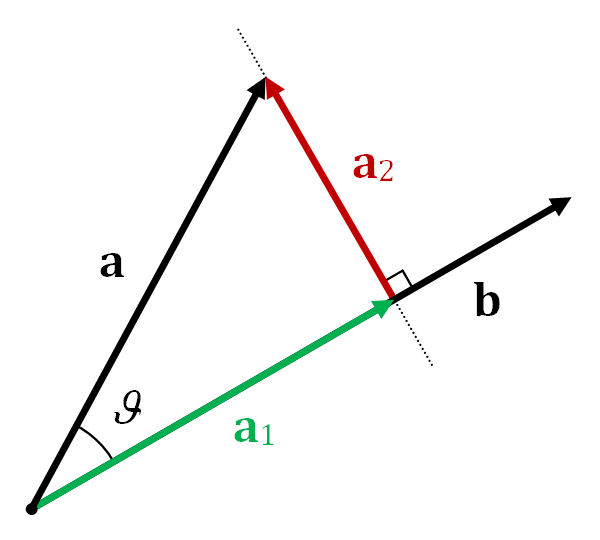
\includegraphics[width=0.3\linewidth]{figures/projection.png}
    \caption{Vector projection}
    \label{fig:projection}
\end{figure}

From that, we have the following equation:
\begin{align*}
    \vv B \cdot (\vv A + \vv \alpha) &= \vv B \cdot \proj_B A \\
    \vv B \cdot (\vv A + \vv \alpha) &= \vv B \cdot (k \vv B) \\
    \vv B \cdot (\vv A + \vv \alpha) &= k (\vv B \cdot \vv B) \\
    \vv B \cdot \vv A + \vv B \cdot \vv \alpha &= \vv B \cdot (k \vv B) \\
    \vv B \cdot \vv A &= \vv B \cdot (k \vv B) & \text{since $\vv\alpha \cdot \vv B = 0$} \\
    k &= \frac{\vv A \cdot \vv B}{\vv B \cdot \vv B}
\end{align*}

Hence,
$$
\proj_B A = \left( \frac{\vv A \cdot \vv B}{\vv B \cdot \vv B} \right) \vv B
$$
In addition, $\comp_B A$ is the norm of $\proj_B A$.
\end{proof}

\section{The Cross Product}
\subsection{Definition}

Recall that the dot product between $A=(x_1,y_1,z_1)$ and $B=(x_2,y_2,z_2)$ is defined as
$$
A \cdot B = x_1x_2+y_1y_2+z_1z_2
$$
but also
$$
A \cdot B = \norm{A}\norm{B}\cos\theta
$$
where $\theta$ is the angle between $A$ and $B$.

The dot product gives us a scalar. We will now define the cross product, which gives us a vector. The cross product $\vv a \times \vv b$ is a vector that is orthogonal to both $\vv a$ and $\vv b$.

\begin{figure}[ht]
    \centering
    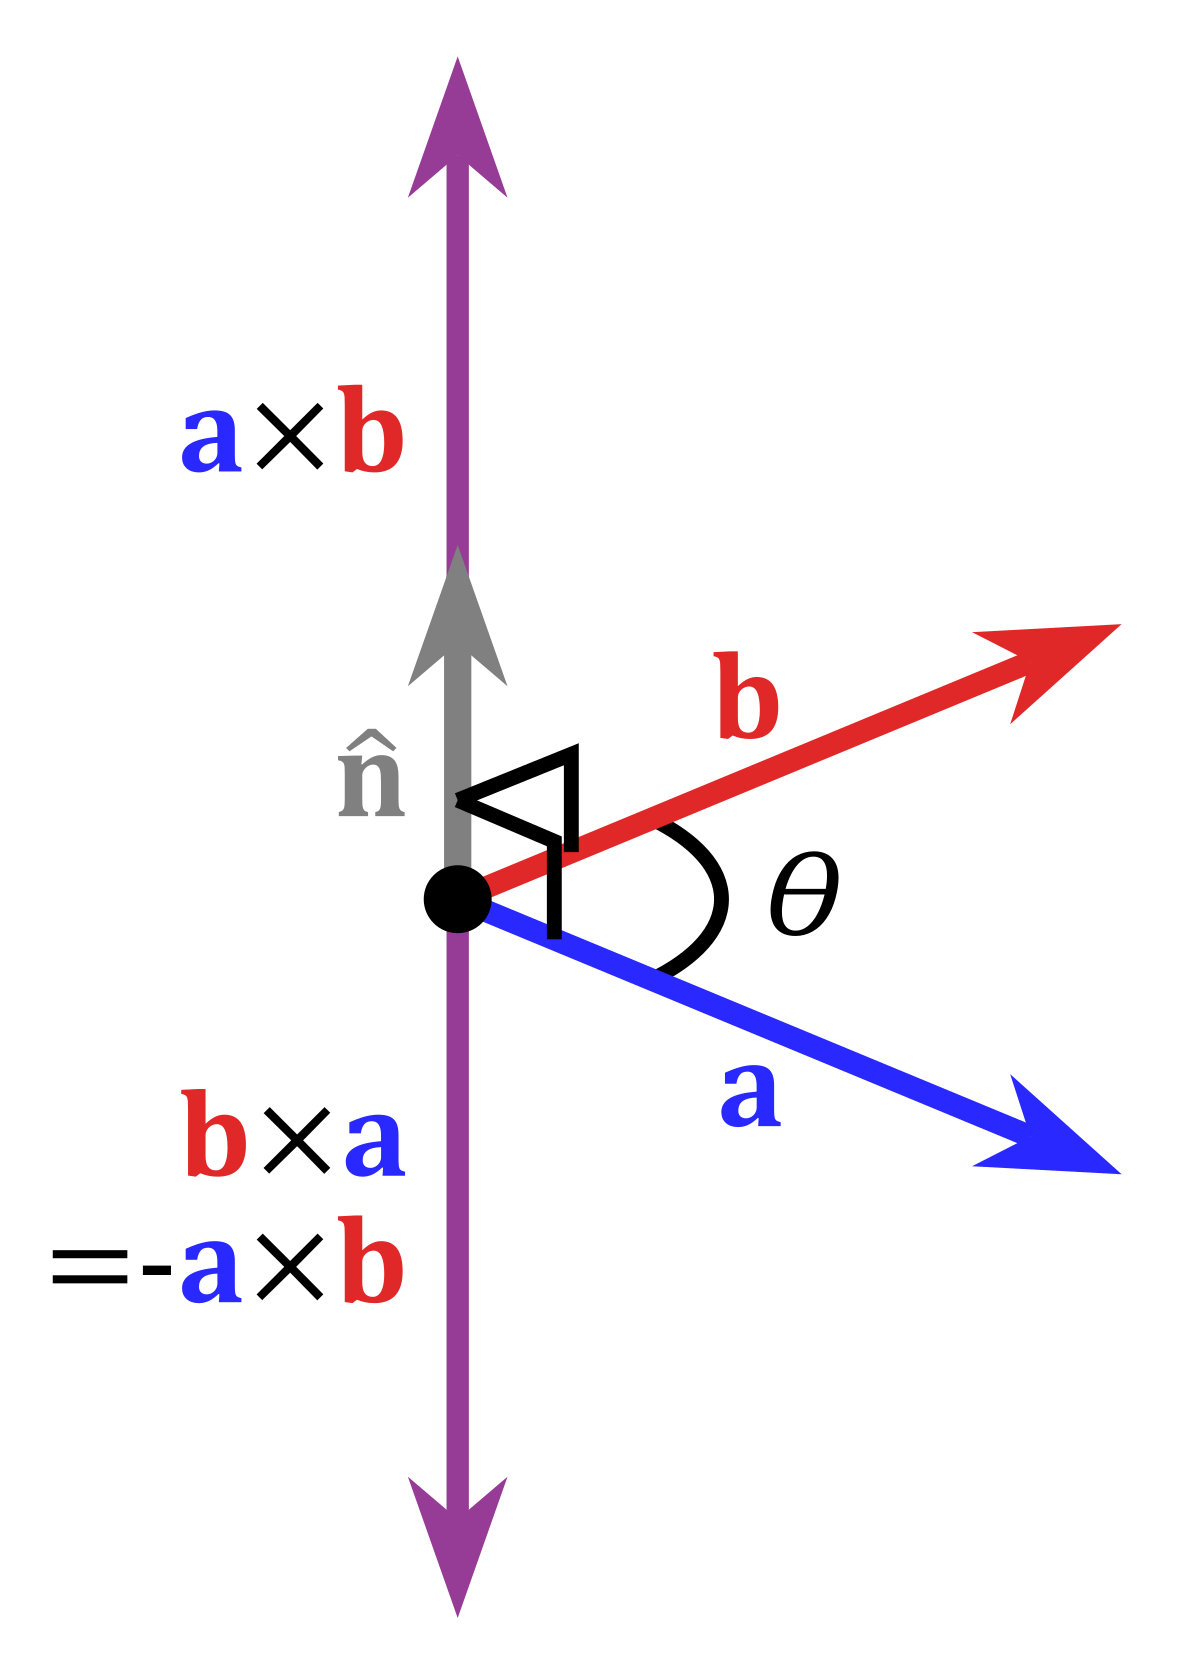
\includegraphics[width=0.3\linewidth]{figures/cross-product.png}
    \caption{The Cross Product}
\end{figure}

Importantly, the cross product is not commutative, i.e. in general, $\vv a \times \vv b \neq \vv b \times \vv a$.

\begin{definition}[The Dot Product]
For vectors $A = (a_1,b_1,c_1)$ and $B=(b_1,b_2,b_3)$ in $\R^3$, 
\begin{align*}
    A \times B &= \begin{vmatrix}
    \vv i & \vv j & \vv k \\
    a_1 & a_2 & a_3 \\
    b_1 & b_2 & b_3
    \end{vmatrix} = \vv i \begin{vmatrix}
    a_2 & a_3 \\
    b_2 & b_3
    \end{vmatrix} - \vv j \begin{vmatrix}
    a_1 & a_3 \\
    b_1 & b_3
    \end{vmatrix} + \vv k \begin{vmatrix}
    a_1 & a_2 \\
    b_1 & b_2
    \end{vmatrix} \\
    &= (a_2b_3-b_2a_3,\, b_1a_3-a_1b_3,\, a_1b_2-b_1a_2)
\end{align*}
\end{definition}

\begin{theorem}
$$
\vv a \times \vv b = \norm{\vv a}\norm{\vv b}\sin\theta
$$
Hence, if $\theta=0$, $\norm{\vv a \times \vv b} = 0$; if $\theta=90$, then $\norm{\vv a \times \vv b}=\norm{\vv a}\norm{\vv b}$; if $\theta=180$, $\norm{\vv a \times \vv b} = 0$.
\end{theorem}

\begin{theorem}[Area of Parallelogram]
The parallelogram defined by the vectors $\vv a, \vv b$ is the norm of their cross product.
$$
A = \norm{\vv a}(\norm{\vv b}\sin\theta) = \norm{\vv a \times \vv b}
$$
\end{theorem}

\subsection{Triple Product}

\begin{definition}
The triple product $\vv a \cdot (\vv b \times \vv c)$ is defined as
$$
\vv a \cdot (\vv b \times \vv c) = \begin{vmatrix}
a_1 & a_2 & a_3 \\
b_1 & b_2 & b_3 \\
c_1 & c_2 & c_3
\end{vmatrix} = (\vv a \times \vv b) \cdot \vv c
$$
\end{definition}

\begin{theorem}
The volume of the parallelepiped determined by vectors $\vv a,\vv b,\vv c$ is the magnitude of the triple product.
$$
V=Ah=\norm{\vv b \times \vv c}\norm{\vv a}|\cos\theta|=\norm{\vv a \cdot (\vv b \times \vv c)}
$$
\end{theorem}

\subsection{Properties}

\begin{multicols}{2}
\begin{enumerate}
    \item $\vv a \times \vv b = - \vv b \times \vv a$
    \item $(c\vv a) \times \vv b = c(\vv a \times \vv b) = \vv a \times (c \vv b)$
    \item $\vv a \times (\vv b + \vv c) = \vv a \times \vv b + \vv a \times \vv c$
    \item $(\vv a + \vv b) \times \vv c = \vv a \times \vv c + \vv b \times \vv c$
    \item $\vv a \cdot (\vv b \times \vv c) = (\vv a \times \vv b) \cdot \vv c$
    \item $\vv a \times (\vv b \times \vv c) = (\vv a \cdot \vv c)\vv b - (\vv a \cdot \vv b)\vv c$
\end{enumerate}
\end{multicols}

\chapter{Geometry of the Euclidean Space}

\section{Lines}

\section{Planes}


\chapter{Vector Functions}

In this chapter, we will study functions of the form
$$
r(t) = \left(f(t),g(t),h(t)\right) = f(t)\vv i + g(t) \vv j + h(t) \vv k
$$
Such function takes in a parameter $t$ and output a vector.

\section{Limit and Continuity}

\begin{definition}[Limit of vector functions]
If $r(t) = (f(t),g(t),h(t))$, then
$$
\lim_{t\to a} r(t) = \left(\lim_{t\to a} f(t),\, \lim_{t\to a} g(t),\, \lim_{t\to a} h(t)\right)
$$
If $\lim_{t\to a} r(t) = r(a)$, then $r$ is continuous at $a$.
\end{definition}

\subsection{Space Curves}
The graph of a vector function is called the space curve. More formally, for the vector function $r(t)=(f(t),g(t),h(t))$, the set $C$ of all points $(x,y,z)$ such that $x=f(t),\; y=g(t),\;z=h(t)$ for $t$ in the domain of the vector function is the space curve.
$$
C = \{ (x,y,z) \in \R^3 \mid x=f(t),\; y=g(t),\;z=h(t) \text{ for some $t \in D$} \}
$$

\begin{example}[Space curves]
\begin{enumerate}
    \item Circle of radius $r$:
    $$
    x=r\cos t, \qquad y=r\sin t, \qquad z=k
    $$
    for $0 \leq t \leq 2\pi$ and some scalar $k \in \R$.
    
    \item Helix
    $$
    x=r\cos t, \qquad y=r\sin t, \qquad z=bt
    $$
    for $b \in \R$. \\
    The helix rises by $2\pi b$ units per turn.
    
    \item Line from the tip of $r_0$ to the end of $r_1$:
    $$
    r(t) = (1-t)\vv{r_0} + t\vv{r_1}
    $$
    for $0 \leq t \leq 1$.
\end{enumerate}

\begin{figure}[ht]
    \centering
    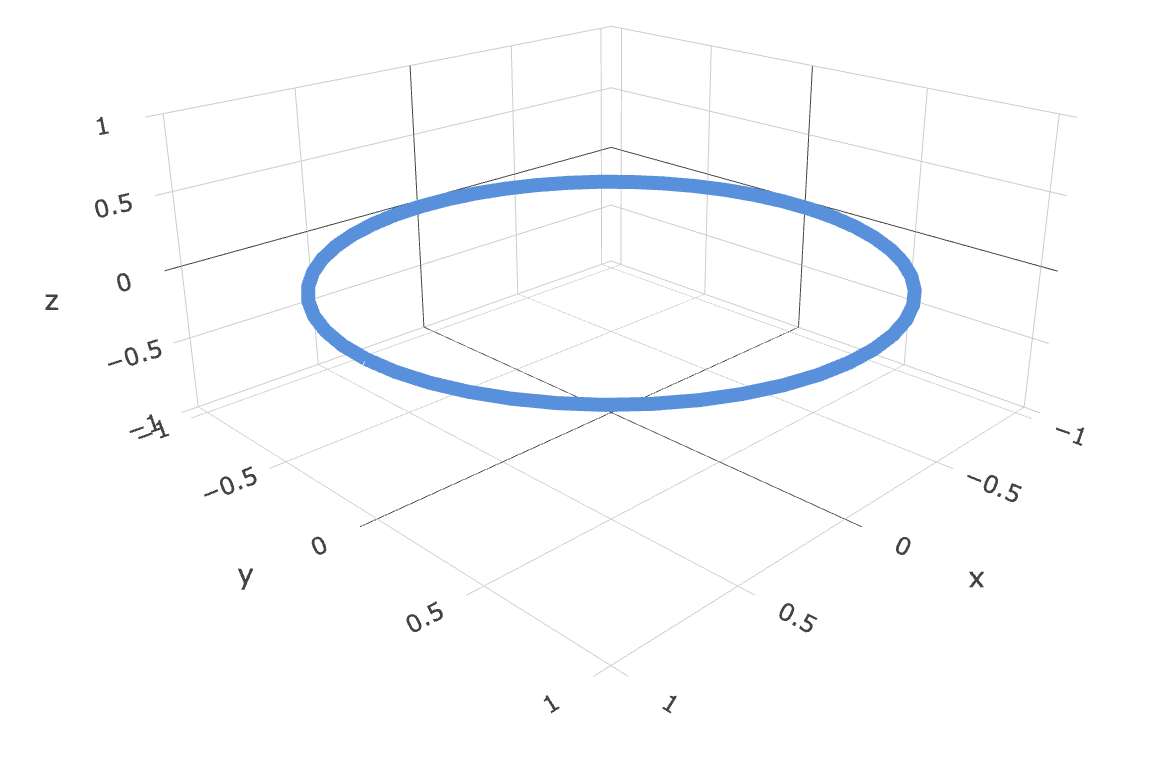
\includegraphics[width=0.3\linewidth]{figures/space-curve-circ.png}
    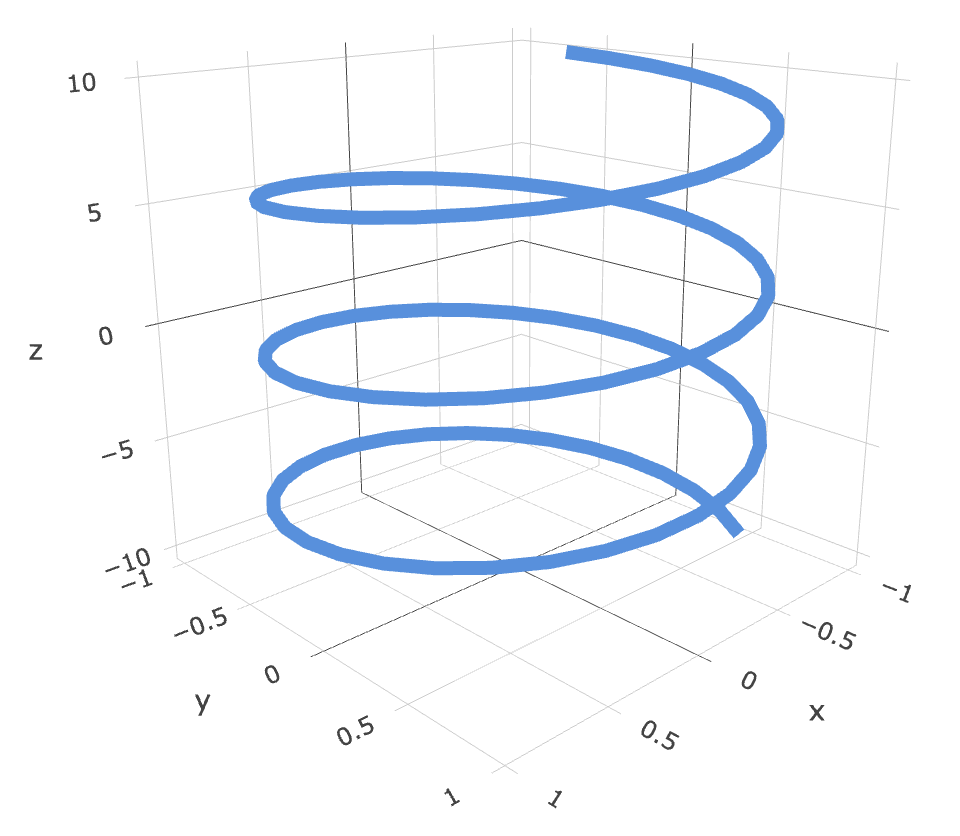
\includegraphics[width=0.3\linewidth]{figures/space-curve-helix.png}
    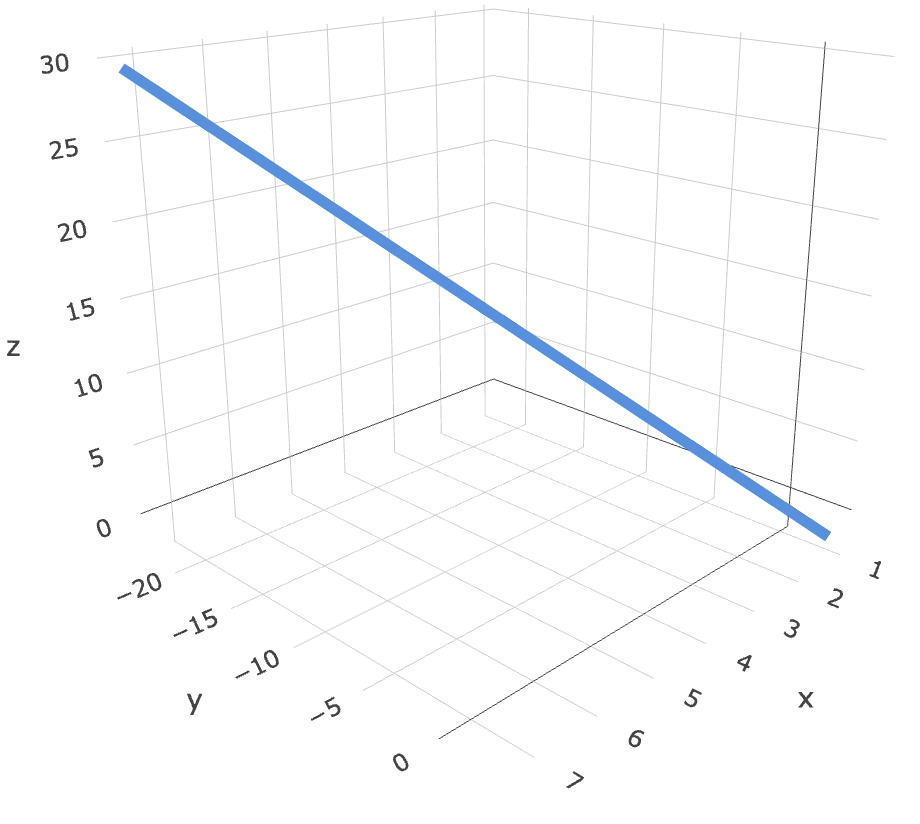
\includegraphics[width=0.3\linewidth]{figures/space-curve-line.png}
    \caption{Examples of space curves}
    \label{fig:space_curves}
\end{figure}
\end{example}

\section{Derivatives and Integrals of Vector Functions}

\subsection{Derivatives}

\begin{definition}[Derivative of vector functions]
$$
\frac{d\mathbf r}{dt} = \mathbf{r}'(t) = \lim_{h\to0}\frac{\mathbf{r}(t+h)-\mathbf{r}(t)}{h}
$$
\end{definition}

If follows from the definition of vector function that
$$
r'(t)= (f'(t),\, g'(t),\, h'(t))
$$

In 2D, the derivative at a point gives us the slope of the tangent line to the graph at that point. Similarly, the derivative of a vector function at a given point gives us a vector that is tangent to the curve.

\begin{figure}[h]
    \centering
    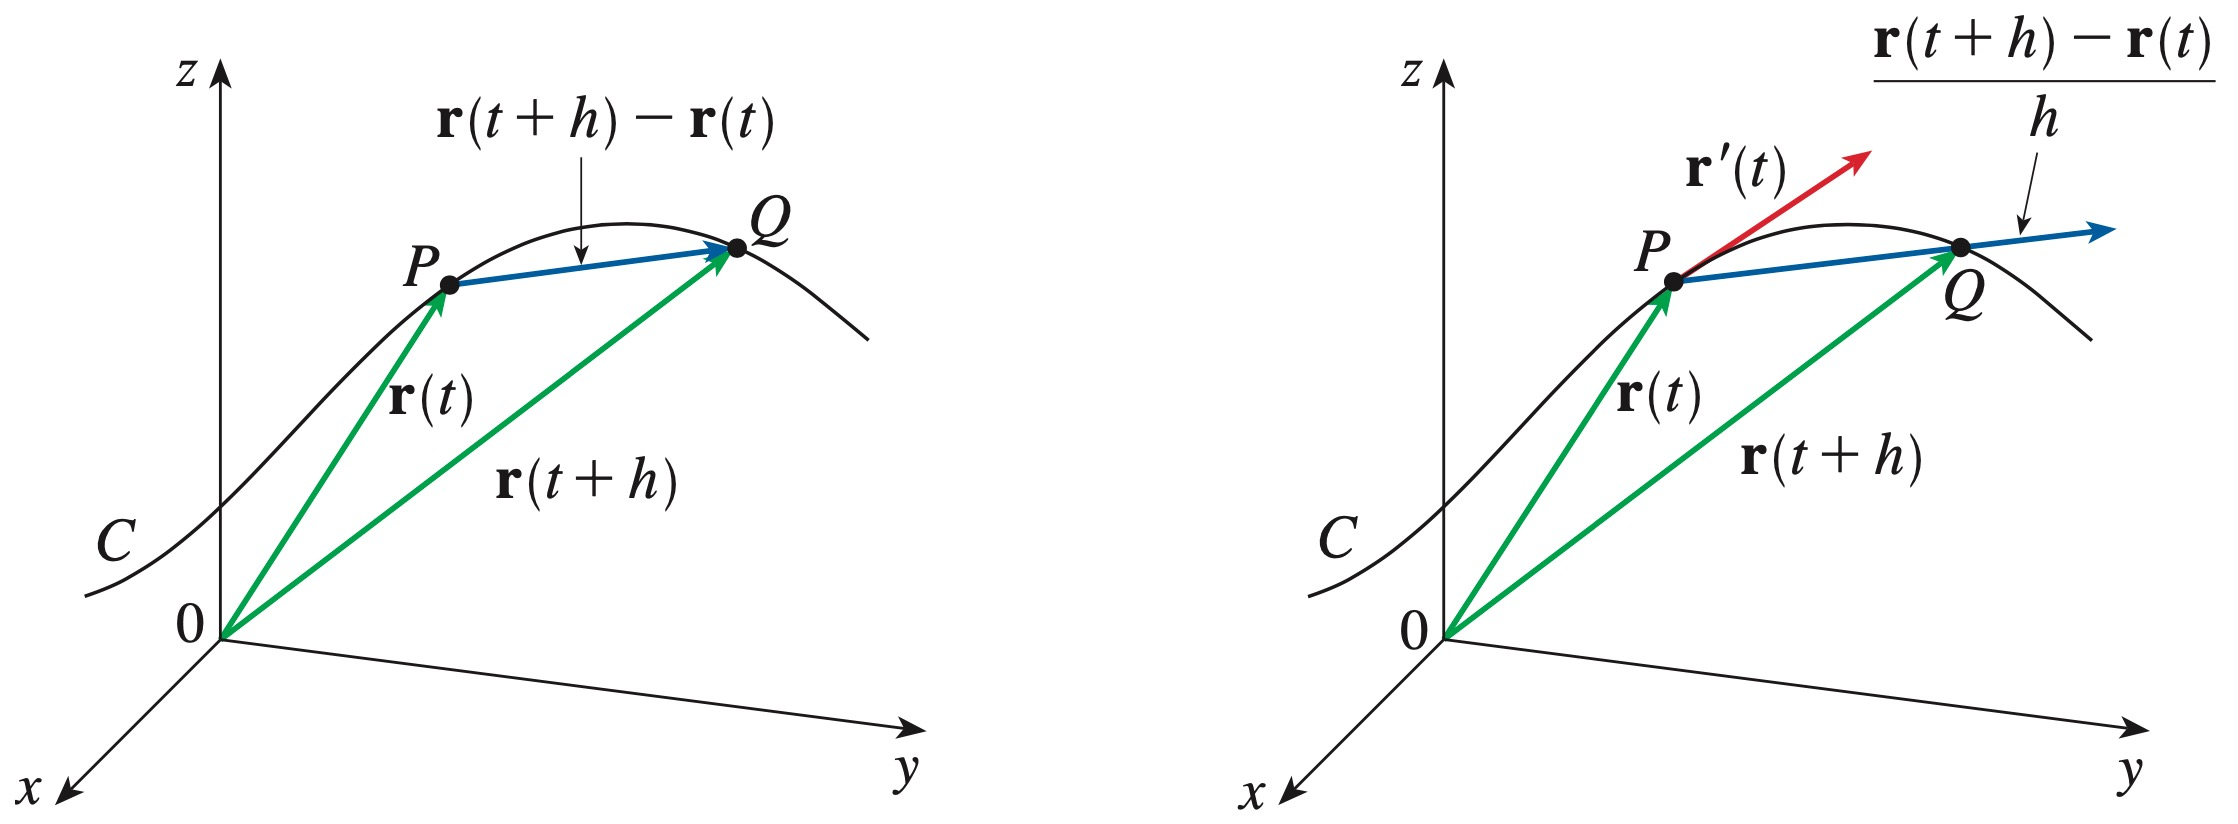
\includegraphics[width=0.6\linewidth]{figures/tangent-vector.jpeg}
    \caption{Secant and tangent vector}
    \label{fig:tan_vec}
\end{figure}

A unit vector that has the same direction as the vector tangent to the curve is called the {\bf unit tangent vector} or simply {\bf tangent vector}, denoted $T$.
$$
T(t) = \frac{r'(t)}{\norm{r'(t)}}
$$

The differentiation rules are mostly the same as real-value functions. There are some variants of the product rule, as shown below:
\begin{theorem}
\begin{multicols}{2}
    \begin{enumerate}
        \item $\displaystyle\frac{d}{dt}\left[ f(t) \mathbf{u}(t) \right] = f'(t)\mathbf{u}(t) + f(t)\mathbf{u}'(t)$
        \item $\displaystyle\frac{d}{dt}\left[ \mathbf{u}(t) \cdot \mathbf{v}(t) \right] = \mathbf{u}'(t)\cdot\mathbf{v}(t) + \mathbf{u}(t)\cdot\mathbf{v}'(t)$
        \item $\displaystyle\frac{d}{dt}\left[ \mathbf{u}(t) \times \mathbf{v}(t) \right] = \mathbf{u}'(t)\times\mathbf{v}(t) + \mathbf{u}(t)\times\mathbf{v}'(t)$
    \end{enumerate}
\end{multicols}
\end{theorem}

\begin{lemma} \label{lem:derivative_sphere}
Let $r(t)$ be a vector function such that $\norm{r(t)}=c$ where $c$ is a constant for all $t$ in the domain. Then, $r(t)$ is orthogonal to $r'(t)$. In other words,
$$
r(t) \cdot r'(t) = 0
$$
\begin{figure}[h]
    \centering
    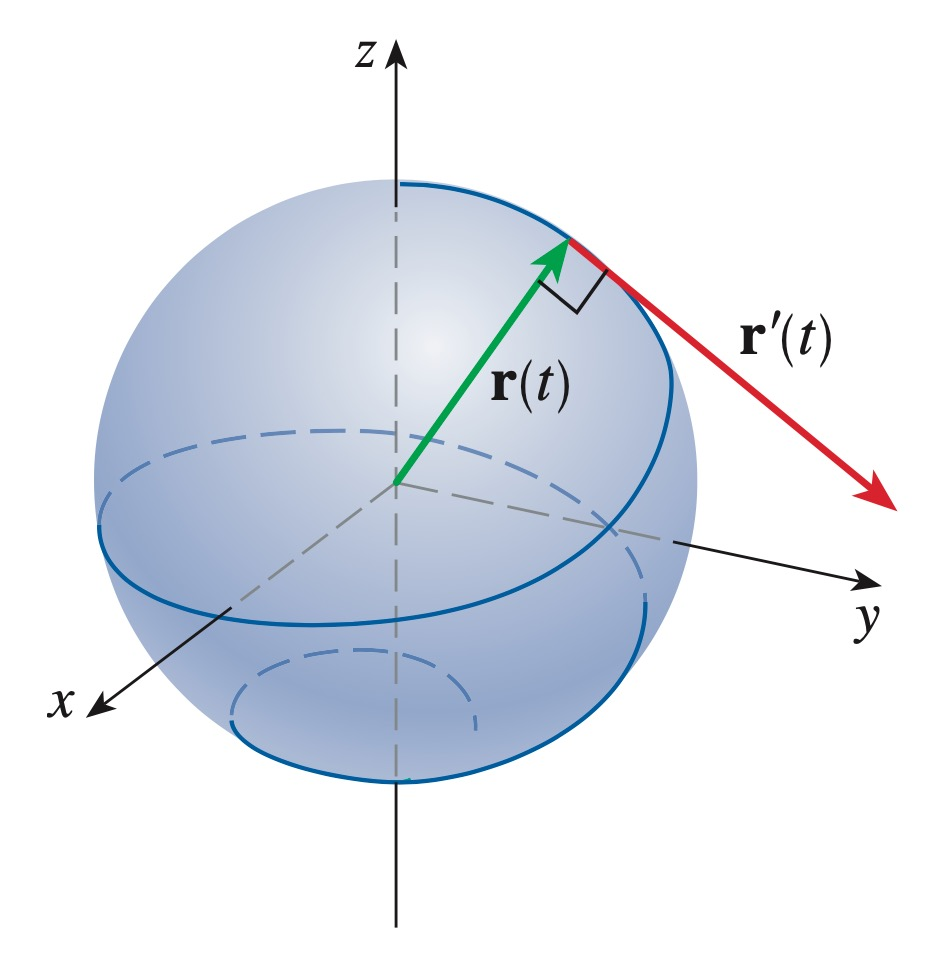
\includegraphics[width=0.3\linewidth]{figures/sphere.jpeg}
    \caption{$r(t)$ will be a function on the surface of a sphere of radius $c$}
    \label{fig:derivative_sphere}
\end{figure}
\end{lemma}

Proof of Lemma \ref{lem:derivative_sphere}

\begin{proof}
\hfill \\
Since $\norm{r(t)} = c$, we can square both sides to get
$$
\norm{r(t)}^2 = c^2
$$
from which we can introduce the dot product
\begin{align*}
    r(t) \cdot r(t) = c^2
\end{align*}
Differentiate both sides
\begin{align*}
    \frac{d}{dt} [r(t) \cdot r(t)] &= \frac{d}{dt} c^2 \\
    r(t) \cdot r'(t) + r'(t) \cdot r(t) &= 0 \\
    2r(t)\cdot r'(t) &= 0 \\
    r(t) \cdot r'(t) &= 0
\end{align*}
\end{proof}

\subsection{Integral}

\begin{definition}[Integral of vector functions]
$$
\int_a^b \mathbf{r}(t)dt = \lim_{n\to\infty}\sum_{i=1}^n \mathbf{r}(t_i^*)\Delta t
$$
\end{definition}
Again, it follows from the definition of vector function that
$$
\int_a^b \mathbf{r}(t)dt = \left(\int_a^b f(t)dt,\; \int_a^b g(t)dt,\; \int_a^b h(t)dt \right)
$$
The integral of a vector function is also a vector. It does not have an obvious geometric meaning.

In physics, we can integrate the acceleration vector to get the velocity vector, and integrate the velocity vector to get the displacement vector.

\section{Arc Length}

Consider each tiny line segment on the curve. Using the Pythagorean's theorem, we know that the length of each segment is
\begin{align*}
    \sqrt{(x_{i+1}-x_i)^2 + (f(x_{i+1}-f(x_i))^2}
\end{align*}
Multiply by $\frac{(x_{i+1}-x_i)}{(x_{i+1}-x_i)}$
\begin{align*}
    (x_{i+1}-x_i) \sqrt{\frac{(x_{i+1}-x_i)^2}{(x_{i+1}-x_i)^2} + \frac{(f(x_{i+1}-f(x_i))^2}{(x_{i+1}-x_i)^2}} \\
\end{align*}
Then, the arc length is just the infinite sum of all infinitely small line segments,
\begin{align*}
    L &=\lim_{n\to\infty} \left[\sum_{i=1}^n (x_{i+1}-x_i) \sqrt{\frac{(x_{i+1}-x_i)^2}{(x_{i+1}-x_i)^2} + \frac{(f(x_{i+1}-f(x_i))^2}{(x_{i+1}-x_i)^2}} \right] \\
    &= \int_a^b \sqrt{1+[f'(x)]^2} dx
\end{align*}
Hence, for 2D parametric curves,
$$
L = \int_a^b \sqrt{\left( \frac{dx}{dt} \right)^2 + \left( \frac{dy}{dt} \right)^2} dt
$$
Similarly, for 3D,
$$
L = \int_a^b \sqrt{\left( \frac{dx}{dt} \right)^2 + \left( \frac{dy}{dt} \right)^2 + \left( \frac{dz}{dt} \right)^2} dt
$$

\begin{theorem}[Arc length]
The arc length between $a$ and $b$ for a vector function (parametric curve) in 3D is
$$
L = \int_a^b \sqrt{\left( \frac{dx}{dt} \right)^2 + \left( \frac{dy}{dt} \right)^2 + \left( \frac{dz}{dt} \right)^2} dt = \int_a^b \norm{\mathbf{r}'(t)}dt
$$
\end{theorem}

\begin{example}
Find the arc length of $r(t) = (\cos\frac{t}{\sqrt 2}, \sin\frac{t}{\sqrt 2}, \frac{t}{\sqrt 2})$ for $0 \leq t \leq 1$.
$$
L = \int_0^2 \norm{r'(t)}dt = \int_0^2 1 dt = 2
$$
\end{example}

\section{Reparameterization w.r.t. Arc Length}

We can change the parameter by transform the domain. Suppose we have $r(t) = (t,2t^2,3t^3)$ for $1 \leq t \leq 5$.

If we define $s = e^t$, then $r(s) = (e,2e^2,3e^3)$ for $0 \leq s \leq \ln 5$. Note that this only works with continuous functions (in this case $e^t$).

Let $s$ be a function that takes $t$ as an input, and outputs the arc length between some point $a$ and $t$. Since 
$$
s(t) = \int_a^t \norm{r'(u)} du
$$
by the Fundamental Theorem of Calculus,
$$
\frac{ds}{dt} = \frac{d}{dt}\int_a^t \norm{r'(u)}du = \norm{r'(t)}
$$

Let $s^{-1}$ be the inverse of $s$ on the relevant interval. Then,
$$
s^{-1}(s(t)) = t \quad \text{ and } \quad s(s^{-1}(s))=s
$$
Differentiate both sides and apply the Chain Rule
$$
\frac{ds}{dt} = \frac{1}{(s^{-1})'(s(t))} \qquad \frac{ds^{-1}}{ds}=\frac{1}{s'(s^{-1}(s))}
$$
Let $q(s)=r(s^{-1}(s))$. $q(s)$ is called the arc length parameterization of $r(t)$.

The arc length parameterization has some really neat properties. Because $ds = \norm{r'(t)}dt$,
$$
L = \int \norm{r'(t)} dt = \int_a^b ds = b-a
$$

To show that $q$ is an arc length parameterization, we just need to show that
$$
\norm{q'(s)} = \left\lVert{\frac{d}{dt} r(s^{-1}(s))}\right\rVert = \norm{(s^{-1})'(s) \cdot r'(s^{-1}(s))} = \left\lVert \frac{r'(s^{-1}(s))}{s'(s^{-1}(s))} \right\rVert = \left\lVert \frac{r'(t)}{r'(t)} \right\rVert = 1
$$

For a vector function parameterized by arc length, the tip of the vector travels at a constant rate of one unit of arc length per unit of time. This is similar to the notion of radian, which is defined as $1 \mathrm{rad} = 1 \text{ unit of arc length}$ in a unit circle.

Despite the nice properties, it is often hard or even impossible to analytically find the arc length parameterization.

\begin{example}[Arc length parameterization]
\begin{enumerate}
    \item Unit circle: $r(t) = (\cos t, \sin t, 0)$. In this case, $r$ is already parameterized with respect to arc length. So, $s=t$, and $r(s) = (\cos s, \sin s, 0)$. This is the definition of radian measure.
    \item Helix: $r(t) = (\cos t, \sin t, t)$. Calculate the arc length:
    $$
    s = \int_0^t \norm{r'(u)}du = \int_0^t \sqrt{\cos^2 u + \sin^2 u + 1} du = \sqrt{2}t
    $$
    Solve for the inverse of $s$, which gives $t= s/\sqrt2$. Hence the arc length parameterization:
    $$
    r(s) = \left( \cos\frac{s}{\sqrt2},\; \sin\frac{s}{\sqrt2},\; \frac{s}{\sqrt2} \right)
    $$
\end{enumerate}
\end{example}

\section{Curvature}

\begin{definition}[Smoothness]
Given a function $r(t)$, a parameterization is called smooth on an interval $I$ if $r'(t) \neq 0$. A curve is called smooth if it has a smooth parameter. A smooth curve has no sharp corners or cusps.
\end{definition}

\begin{definition}[Curvature]
The curvature of a curve is
$$
\kappa = \left\lVert{\frac{dT}{ds}}\right\rVert
$$
\end{definition}

Notice that $\kappa$ depends on the arc length parameterization. We can calculate this number as
$$
\frac{dT}{ds} = \frac{dT}{ds} \cdot 1 = \frac{dT}{ds}\cdot \frac{dt}{dt} = \frac{dT}{dt} \cdot \frac{dt}{ds}
$$
Since $ds/dt = \norm{r'(t)}$,
$$
\frac{dT}{ds} = \frac{dT/dt}{ds/dt} = \frac{dT/dt}{\norm{r'(t)}}
$$
Hence,
$$
\kappa = \frac{\norm{dT/dt}}{\norm{r'(t)}}
$$
which is now independent of the arc length parameterization $s$.

\begin{example}
The curvature of a circle of length $a$.

The equation of that circle is $r(t) = (a\cos t, a\sin t)$. Therefore, $r'(t)=(-a\sin t,a \cos t)$ and $\norm{r'(t)}=a$.

So,
$$
T(t)=\frac{r'(t)}{\norm{r'(t)}} = (-\sin t, \cos t)
$$
and
$$
T'(t)=(-\cos t, -\sin t)
$$
This gives $\norm{T'(t)} = 1$ and hence
$$
\kappa = \frac{T'(t)}{r'(t)} = 1/a
$$
This result also implies that circle has constant curvature, and that smaller circle has larger curvature.
\end{example}

\begin{theorem} \label{eq:alt_curvature}
The curvature can also be calculated as follows:
$$
\kappa(t) = \frac{\norm{r'(t) \times r''(t)}}{\norm{r'(t)}^2}
$$
and for plane curves of the form $y = f(x)$, we can choose $x$ as the parameter and write $r(x) = (x,f(x))$. Then,
$$
r'(x) = (1, f'(x)) \qquad r''(x)=(0,f''(x))
$$
And $\norm{r'(x)} = \sqrt{1+[f'(x)]^2}$. Hence, by the previous equation \eqref{eq:alt_curvature}
$$
\kappa(x) = \frac{\norm{f''(x)}}{\left[ 1+(f'(x))^2 \right]^{3/2}}
$$
\end{theorem}

\section{Normal and Binormal Vectors}

\begin{definition}[Normal vector]
Given a function $r(t)$, we know that $T(t) = \frac{r'(t)}{\norm{r'(t)}}$ is a unit vector called the tangent vector. Recall that by Lemma \ref{lem:derivative_sphere} if $\norm{r(t)}=c$ where $c$ is a constant, then $r(t)\cdot r'(t) = 0$.

Since $\norm{T(t)}=1$, we can conclude that $T(t)$ is perpendicular to $T'(t)$. We define the (unit) normal vector as
$$
N(t) = \frac{T'(t)}{\norm{T'(t)}}
$$
which is normal to $T(t)$.
\end{definition}

\begin{definition}[Binormal vector]
We define the binormal vector $B$ as the cross product between $T$ and $N$.
$$
B(t) = T(t) \times N(t)
$$
which is also a unit vector so $\norm{B(t)}=1$.
\end{definition}

\begin{figure}[h]
    \centering
    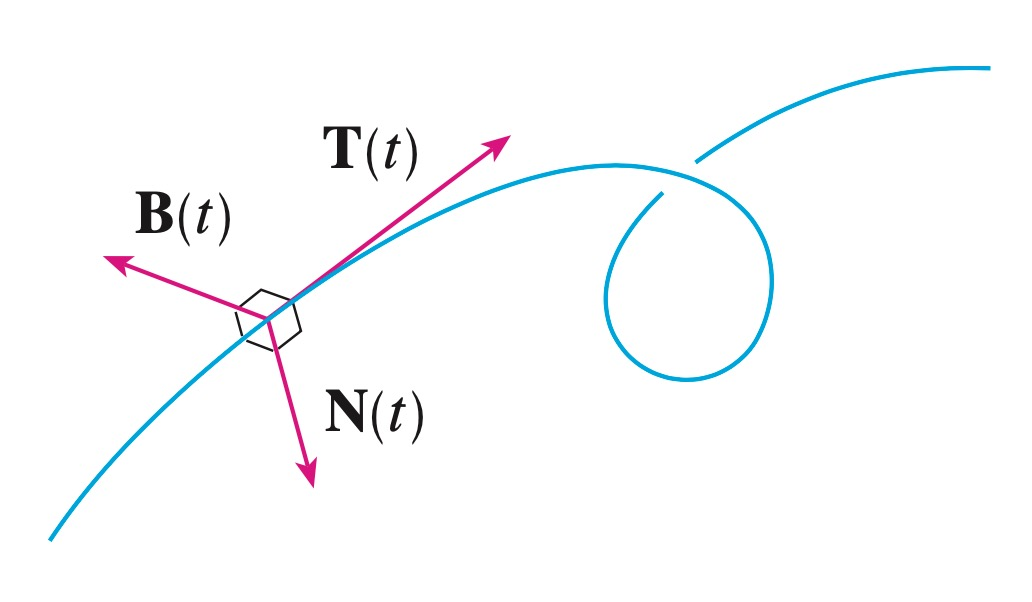
\includegraphics[width=0.3\linewidth]{figures/normal-binormal.jpeg}
    \caption{Normal and Bionormal function}
    \label{fig:normal_binormal_vec}
\end{figure}

$T,N,B$ together define a new set of axes. $B$ defines the binormal line, and $N$ defines the normal line.

In addition, the plane between $N$ and $T$ is called the osculating plane. The plane between $B$ and $T$ is called the rectifying plane. The plane between $N$ and $B$ is called the normal plane.

\begin{figure}[h]
    \centering
    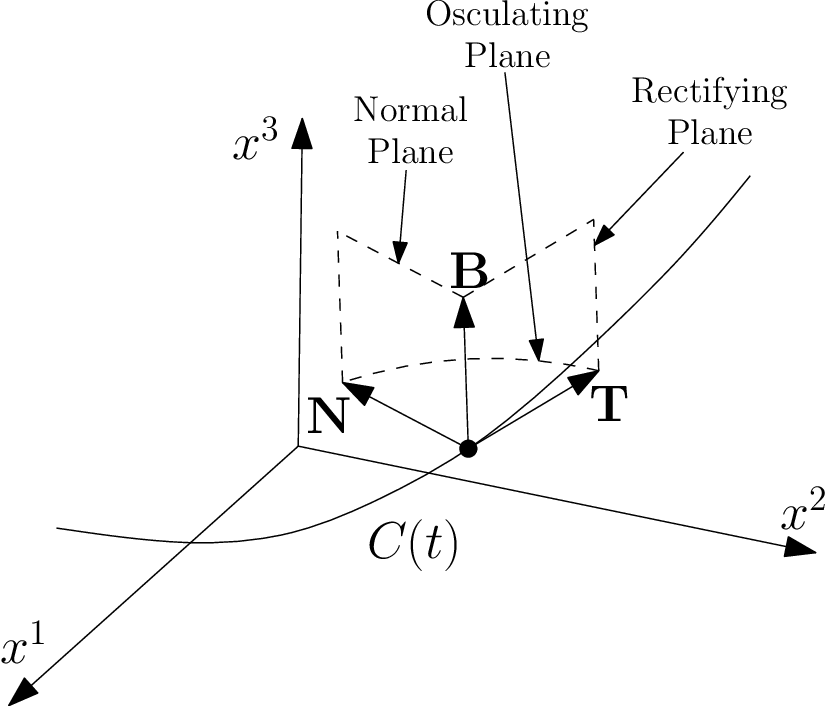
\includegraphics[width=0.4\linewidth]{figures/NTB-planes.png}
    \caption{Normal, osculating, and rectifying planes}
    \label{fig:NTB_planes}
\end{figure}

\section{Torsion}

\chapter{Topology of $\R^n$}

\section{Open and Closed Subsets}

\section{Compactness}

\section{EVT}

\section{IVT}

\chapter{Functions of Multiple Variables}

\section{Multivariable Functions}

In this chapter, we study function of the form
$$
f:\, \R^2 \to \R
$$
or equivalently $f:\, \R\times\R \to \R$.

Those are functions of two variables. The graph of function of two variables is defined as
$$
\{ (x,y,z) \in \R^3 \mid z = f(x,y) \}
$$

\section{Level Curves}

\section{Limit and Continuity}



\chapter{Derivatives}

\section{Partial Derivatives}

\begin{definition}[Partial derivative]
Given a function $f(x,y)$, we want to define a derivative for $f(x,y)$. Since we have two variables, we can define the derivative using only one of them. Recall that for functions of one variable:
$$
f'(a) = \lim_{h\to 0}{\frac{f(a+h)-f(a)}{h}} \qquad \text{provided that the limti exists.}
$$
If we fix the value of $y$ and we use values $(x,y)$ to approach $(a,b)$, we define the partial derivative of $f(x,y)$ with respect to $x$ as
$$
\partialderiv{}{x} f(x,y) = \lim_{h\to0}\frac{f(x+h,y)-f(x,y)}{h}
$$
Similarly, if $x$ is fixed, the partial derivative with respect to $y$ can be defined as
$$
\partialderiv{}{y} f(x,y) = \lim_{h\to0}\frac{f(x,y+h)-f(x,y)}{h}
$$
provided that the limits exist.
\end{definition}

There are different ways to denote the partial derivative
$$
f_x =   f_x(x,y) = \partialderiv{f}{x} = \partialderiv{}{x}f(x,y)
$$

\section{Tangent Plane}

\subsection{Definition}
Given $f(x,y)$ and point $(a,b,c)$ on the surface, the plane tangent to the surface at $(a,b,c)$ is
$$
z-c = f_x(a,b)(x-a) + f_y(a,b)(y-b)
$$

\subsection{Linear Approximation}
Differentiable functions are locally linear, meaning that if zoom in close enough, the function will appear to be linear. Because of that, we can approximate the value of the function near $(a,b)$ using the tangent plane at that point.

Let $L$ be the linear function that is the tangent plane at point $(a,b)$.
$$
L(x,y) = f(a,b) + f_x(a,b)(x-a) + f_y(a,b)(y-b)
$$
$L$ is called the linearization of $f$ at $(a,b)$, and we can use that to approximate the value of $f$ at points near $(a,b)$.
$$
f(x,y) \approx f(a,b) + f_x(a,b)(x-a) + f_y(a,b)(y-b)
$$

\section{Higher Order Derivatives}

\begin{theorem}[Clairaut's Theorem (symmetry of second derivatives)]
Suppose that $S \subseteq \R^n$ is open. If $f\; S \to \R$ is twice continuously differentiable (of class $C^2$), then
$$
\frac{\partial^2 f}{\partial x_i \partial x_j} = 
\frac{\partial^2 f}{\partial x_j \partial x_i}
$$
for all $i,j=1,\cdots, n$ everywhere in $S$.
\end{theorem}

The proof of the Clairaut's Theorem utilizes the Mean Value Theorem.

We can expand the Clairaut's Theorem to higher-order derivatives.

\begin{theorem}
Suppose that $S$ is an open subset of $\R^n$ and that $f:\;S \to \R$ is of class $C^k$. For any integers $i_1,\cdots,i_k$ between $1$ and $n$, if $j_1,\cdots,j_k$ is a reordering of $i_1,\cdots,i_k$, then
$$
\frac{\partial}{\partial x_{i_k} }\cdots 
\frac{\partial}{\partial x_{i_1} }f
\ = \ 
\frac{\partial}{\partial x_{j_k} }\cdots 
\frac{\partial}{\partial x_{j_1} }f
$$
everywhere in $S$.
\end{theorem}
This theorem can be proved from the Clairaut's Theorem using induction.

\section{The Chain Rule}

\subsection{Review: Chain rule for single-variable functions}
For $f(x)$ where $x=g(t)$
$$
\frac{df}{dt} = \frac{df}{dx}\frac{dx}{dt}
$$
or equivalently
$$
\frac{df}{dt} = f'(g(t)) \cdot g'(t)
$$

\subsection{Multivariable Chain Rule}

\begin{theorem}[The Chain Rule - 1]
If $f(x,y)$ is a function and $x=g(t)$ and $y=h(t)$, then
$$
\frac{df}{dt} = \partialderiv{f(x,y)}{x} \frac{dx}{dt} + \partialderiv{f(x,y)}{y} \frac{dy}{dt}
$$
\end{theorem}

\begin{theorem}[The Chain Rule - 2]
Suppose that $z=f(x,y)$ is a differentiable function of $x$ and $y$, where $x = g(s,t)$ and $y=h(s,t)$ are differentiable functions of $s$ and $t$. Then
$$
\partialderiv{z}{s} = \partialderiv{z}{x}\partialderiv{x}{s} + \partialderiv{z}{y}\partialderiv{y}{s} \qquad \partialderiv{z}{t} = \partialderiv{z}{x}\partialderiv{x}{t} + \partialderiv{z}{y}\partialderiv{y}{t}
$$
\end{theorem}

\begin{center}
    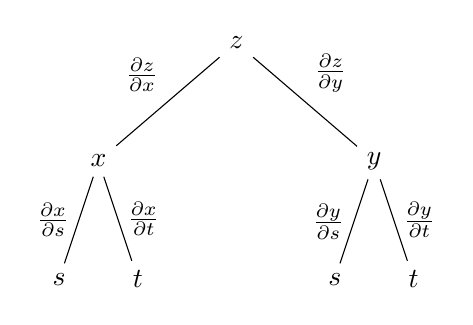
\begin{tikzpicture}[level distance=1.5cm,
    level 1/.style={sibling distance=3.5cm},
    level 2/.style={sibling distance=1cm}]
    \node {$z$}
        child {  
            node {$x$}
            child {
                node {$s$}
                edge from parent node[left,draw=none] {$\partialderiv{x}{s}$}
            }
            child {
                node {$t$}
                edge from parent node[right,draw=none] {$\partialderiv{x}{t}$}
            }
            edge from parent node[above left,draw=none] {$\partialderiv{z}{x}$}
        }
        child {  
            node {$y$}
            child {
                node {$s$}
                edge from parent node[left,draw=none] {$\partialderiv{y}{s}$}
            }
            child {
                node {$t$}
                edge from parent node[right,draw=none] {$\partialderiv{y}{t}$}
            }
            edge from parent node[above right,draw=none] {$\partialderiv{z}{y}$}
        };
    \end{tikzpicture}
\end{center}

\begin{theorem}[The Chain Rule - General Case]
Suppose that $u$ is a differentiable function of the $n$ variables $x_1, x_2, \cdots , x_n$ and each $x_j$ is a differentiable function of the $m$ variables $t_1, t_2, \cdots , t_m$. Then $u$ is a function of $t_1, t_2, \cdots, t_m$ and
$$
\partialderiv{u}{t_i} = \partialderiv{u}{x_1}\partialderiv{x_1}{t_i} + \cdots + \partialderiv{u}{x_n}\partialderiv{x_n}{t_i} = \sum_{j=1}^n \partialderiv{u}{x_j}\partialderiv{x_j}{t_i}
$$
\end{theorem}

\subsection{Generalization}
We can further generalize the Chain Rule using Jacobian matrix and matrix multiplication.

If $\mathbf g$ is differentiable at $\mathbf a$, and $\mathbf f$ is differentiable at $\mathbf{g}(\mathbf{a})$, then the composite function $\mathbf f \circ \mathbf g$ is differentiable at $\mathbf a$ and
$$
D(\mathbf f\circ\mathbf g)(\mathbf a) = [D\mathbf f(\mathbf g(\mathbf a))] \ [D\mathbf g(\mathbf a)].
$$
where $D\mathbf f$ denotes the Jacobian of $\mathbf f$
$$
D\mathbf f = \left[ \partialderiv{\mathbf f}{x_1}, \cdots, \partialderiv{\mathbf f}{x_2} \right]
$$
Writing this as individual components and partial derivatives gives
$$
\frac {\partial }{\partial x_j} (f_k\circ \mathbf g)(\mathbf a) 
=\sum_{i=1}^m \frac{\partial f_k}{\partial y_i}(\mathbf g(\mathbf a)) \ \frac{\partial g_i}{\partial x_j}(\mathbf a)
$$

\section{Differentiability}

\subsection{Definitions}

\begin{definition}[Differentiability for single variable]
If $z=f(x)$, then $f$ is differentiable at $x$ if there exists $m$ and $\epsilon$ such that $\Delta z$ can be expressed in the form
$$
\Delta z = f(x+h)-f(x) = mh + \epsilon h \qquad \text{ and } \qquad \lim_{h \to 0} \frac{\epsilon h}{h} = \lim_{h\to 0} \epsilon = 0
$$
The value of $m$ is the derivative of $f$ evaluated at $x$ (i.e. $f'(x)=m$).
\end{definition}

This equivalent definition can be understood as follows: temporarily fix $x$, treat $h$  as a variable, and view $\Delta z = f(x+h)-f(x)$ as a function of $h$. Then $f$ is differentiable at $h$ if $\Delta z$ is approximately $mh$, with an error term $\epsilon h$ that approaches zero as $h \to 0$.

In other words, this definition says that a function is differentiable if the linear approximation of the function is a good approximation at $x$ when for values close to $x$.

\begin{figure}[h]
    \centering
    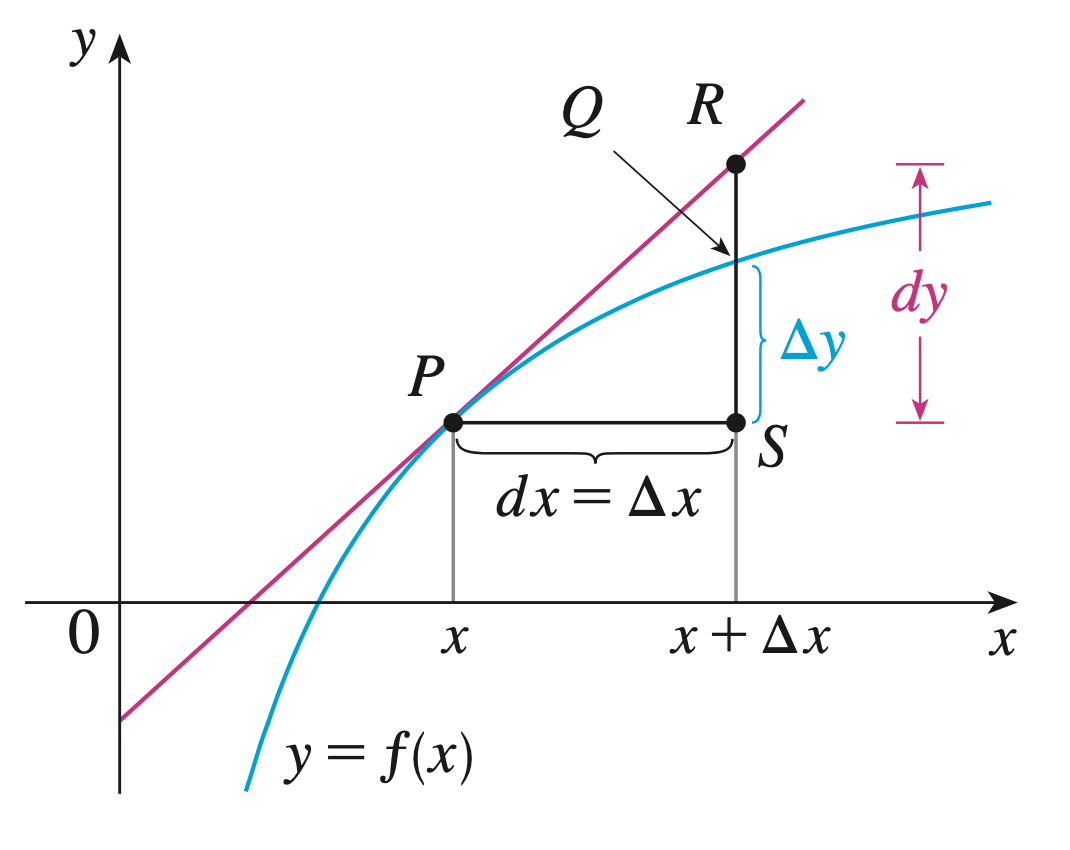
\includegraphics[width=0.4\linewidth]{figures/linear-appox.png}
    \caption{Linear approximation}
    \label{fig:linear-approx}
\end{figure}

We can extend this definition to functions with multiple variables.

\begin{definition}[Differentiability for multiple variables]
If $z=f(x,y)$, then $f$ is differentiable at $(x,y)$ if there exists $m,n$ and $\epsilon_1, \epsilon_2$ such that $\Delta z$ can be expressed in the form
$$
\Delta z = m \Delta z + n \Delta y + E_1(\Delta x) + E_2(\Delta y)
$$
and $\epsilon_1 \to 0, \epsilon_2 \to 0$ as $(\Delta x, \Delta y) \to (0,0)$. $m=f_x(x,y)$ and $n=f_y(x,y)$.
\end{definition}

Alternatively, this can be phrased using vectors.
\begin{definition}
Suppose that $f$ is a function. We say that $f$ is differentiable at $x \in \R^n$ if there exists a vector $\vv m \in \R^n$ such that
$$
f(\vv x + \vv h) - f(\vv x) = \vv m \cdot \vv h + E(\vv h)
$$
where $\displaystyle \lim_{\vv h \to 0} \frac{E(\vv h)}{\norm{\vv h}} = 0$.

When this holds, we define $\nabla f(\vv x) = \vv m$
\end{definition}

\subsubsection{Partial Differentiability}

\begin{theorem}[Differentiability implies partial differentiability]
Let $f$ be a function. If $f$ is differentiable at a point $\vv x \in \R^n$, then $\partialderiv{f}{x_j}$ exists for all $j = 1,\cdots, n$, and in addition,
$$
\nabla f(\vv x) = \left(\partialderiv{f}{x_1},\cdots,\partialderiv{f}{x_n}\right)(\vv x)
$$
The converse is NOT true.
\end{theorem}

This theorem can be helpful when determining the differentiability of a function:
\begin{itemize}
    \item If any partial derivative does not exist, then $f$ is not differentiable
    \item If all partial derivative exist, then $\vv m = (\partialderiv{f}{x_1},\cdots,\partialderiv{f}{x_n})$ is the only possible vector that may work in the definition of differentiability.
\end{itemize}

\section{Directional Derivative and Gradient}

\subsection{Directional Derivative}

The directional derivative of $f$ at $(x_0,y_0)$ in the direction of a unit vector $\vv u = (a,b)$ is
$$
\partial_u f(x_0,y_0) = \lim_{h \to 0} \frac{f(x_0+ha, y_0+hb) - f(x_0,y_0)}{h}
$$
provided that the limit exists.

More generally,
$$
\partial_u f(\vv x) = \lim_{h\to 0} \frac{f(\vv x + h\vv u) - f(\vv x)}{h}
$$

\begin{theorem}
If $f$ is differentiable at a point $\vv x$, then $\partial_u f(\vv x)$ exists for every unit vector $\vv u$, and moreover,
$$
\partial_u f(\vv x) = \vv u \cdot \nabla f(\vv x) = \sum_{j=1}^n \partialderiv{f}{x_j}u_j
$$
\end{theorem}

The directional derivative tells us the instantaneous rate of change of the surface at point $\vv x$ in the direction of the unit vector $\vv u$.

\begin{figure}[h]
    \centering
    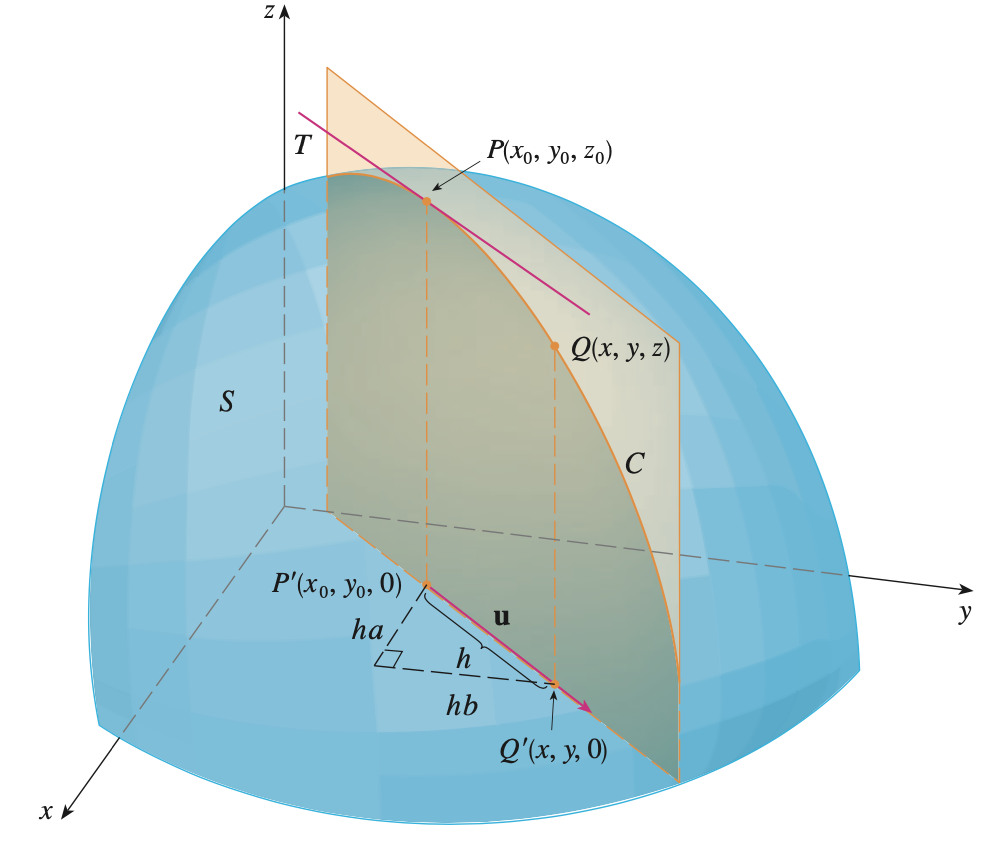
\includegraphics[width=0.5\linewidth]{figures/direcitonal-derivative.png}
    \caption{Directional derivative at $\protect P$ is the slope of the tangent line $\protect T$ to $\protect C$. $\protect C$ is the curve obtained by intersecting the surface with a plane in the direction of $\protect \vv u$}
    \label{fig:directional-derivative}
\end{figure}

In particular, we can see that the partial derivative can be written in terms of directional derivatives. For any $j \in \{1,\cdots,n \}$
$$
\partialderiv{f}{x_j} = \partial_{\hat{e_j}}f
$$
where $\hat{e_j}$ denotes the unit vector in the $j$-th coordinate direction.

\subsection{Gradient}

We defined gradient in the definition of differentiability. We now formally define gradient in terms of partial derivatives.

\begin{definition}[Gradient]
If $f$ is a function, then the gradient of $f$ is the vector function $\nabla f$ defined by
$$
\nabla f(x,y) = \partialderiv{f}{x}\vv i + \partialderiv{f}{y}\vv j
$$
More generally,
$$
\nabla f(\vv x) = \left(\partialderiv{f}{x_i},\cdots,\partialderiv{f}{x_n}\right) (\vv x)
$$
\end{definition}

\begin{theorem}
If it is not zero, $\nabla f(\vv x)$ points in the direction where $f$ has the greatest increase.

\begin{proof}
Since
$$
\partial_u f = \nabla f \cdot \vv u = \norm{\nabla f}\norm{\vv u}\cos\theta = \norm{\nabla f}\cos\theta
$$
The maximum value of $\cos\theta$ is $1$, which occurs when $\theta = 0$. Therefore, the maximum value $\partial_u f$ is $\norm{\nabla f}$ and it occurs when $\theta = 0$, that is when $\vv u$ has the same direction as $\nabla f$.
\end{proof}
\end{theorem}

\section{Maximum and Minimum Values}

\begin{definition}[Critical points]
If $S$ is an open subset of $\R^n$ and $f:\, S \to \R$ is differentiable, then a point $a \in S$ is a critical point if $\nabla f(a)=\vv 0$.
\end{definition}

\subsection{First derivative test}

\begin{theorem}[First derivative test]
If $f$ is differentiable, then every local extremum is a critical point.
\end{theorem}

\subsection{Second derivative test}

\begin{theorem}[Second derivative test]
Suppose the second partial derivatives of $f$ are continuous on a disk with center $(a,b)$, and suppose that $f_x(a,b)=0$ and $f_y(a,b)=0$. Let,
$$
D= D(a,b) = f_{xx}(a,b) f_{yy}(a,b) - [f_{xy}(a,b)]^2
$$
Then
\begin{itemize}
    \item If $D>0$ and $f_{xx}(a,b) > 0$, then $f(a,b)$ is a local minimum
    \item If $D>0$ and $f_{xx}(a,b) < 0$, then $f(a,b)$ is a local maximum
    \item If $D<0$ then $(a,b)$ is a saddle point of $f$
    \item If $D=0$, the test is inconclusive
\end{itemize}
\end{theorem}

\subsection{A More Technical Formulation of the Second Derivative Test}

\subsubsection{Hessian Matrix}
\begin{definition}[Hessian matrix]
$$
H = Hf= \left(\begin{array}{ccc}
\partial_1\partial_1 f & \cdots & \partial_1\partial_n f \\
\vdots & \ddots & \vdots \\
\partial_n\partial_1 f & \cdots & \partial_n\partial_n f 
\end{array}
\right)
$$
For example, for functions of two variables, the Hessian matrix is defined as
$$
H = Hf= \left(\begin{array}{ccc}
\partial_x\partial_x f & \partial_x\partial_y f \\
\partial_y\partial_x f & \partial_y\partial_y f
\end{array}
\right) =
\left(\begin{array}{ccc}
f_{xx} & f_{xy} \\
f_{yx} & f_{yy}
\end{array}
\right)
$$
\end{definition}

\subsubsection{Properties of Symmetric Matrices}

Given a symmetric $n\times n$ matrix with entries $a_{ij}$ for $i,j \in \{1,\cdots, n\}$, we can define a function $\R^n \to \R$
$$
\vv x \mapsto (A\vv x)\cdot \vv x = \sum_{i,j=1}^n a_{ij}x_ix_j
$$

\begin{definition}[Definite matrices]
A symmetric $n\times n$ matrix is
\begin{itemize}
    \item positive definite if $\vv x^\top A \vv x > 0$ for all $\vv x \neq 0$
    \item nonnegative definite if $\vv x^\top A \vv x \geq 0$ for all $\vv x \in \R^n$
\end{itemize}
In addition, we say that $A$ is
\begin{itemize}
    \item negative definite if $-A$ is positive definite
    \item nonpositive definite if $-A$ is nonnegative definite
\end{itemize}
Otherwise if none of the above holds, the we say that $A$ is indefinite. Equivalently, $A$ is indefinite if
$$
\exists \vv x, \vv y \in \R^n,\; \vv x^\top A \vv x < 0 < \vv y^\top A \vv y
$$
\end{definition}

\chapter{Integrals}

\section{Darboux Integral}

\subsection{Rectangles and Partitions}
\begin{definition}[Rectangle]
A rectangle $R \subseteq \R^n$ is a set defined by
$$
R = [a_1,b_1] \times [a_2, b_2] \times \cdots \times [a_n, b_n]
$$
for some $a_1<b_1,\;\cdots a_n < b_n$.
\end{definition}

\begin{definition}[Partition of Interval]
Given a closed interval $[a,b]$ of $\R$, a partition of $[a,b]$ is a finite collection $P \subseteq [a,b]$ of points of $[a,b]$ that includes the points $a$ and $b$.
$$
a = t_0 < t_1 < \cdots < t_k = b
$$
\end{definition}

\begin{definition}[Partition of Rectangle]
Given a rectangle $R = [a_1,b_1] \times [a_2, b_2] \times \cdots \times [a_n, b_n]$, the partition of $R$ is an $n$-tuple $P=(P_1,\cdots,P_n)$ where $P_i$ is a partition of $[a_i,b_i]$. Intuitively, we break the rectangle $R$ into finitely many subrectangles.

If $P_i$ contains $k_i$ many subintervals, then the partition $P$ of $R$ contains $\prod_{i=1}^n k_i$ many subrectangles.
\end{definition}

\subsection{Refinement}

\begin{definition}[Refinement]
If $P$ and $Q$ are two partitions of a rectangle $R$. We say that $Q$ is a refinement of $P$ if
$$
\forall i,\; Q \subset P'
$$
\end{definition}

\begin{lemma}[Common Refinement]
Given two partitions $P$ and $Q$, one can always find a partition $O = P \cup Q$ that is finer than both $P$ and $Q$.
\end{lemma}

\begin{lemma}
If $Q$ is a refinement of $P$, then
$$
L_Q f \geq L_P f \qquad U_Q f \leq U_Q f
$$
\end{lemma}

\begin{lemma}
For every two partitions $P$ and $Q$,
$$
L_P f \leq U_Q f
$$
\end{lemma}

All these three lemmas were proven when we were first introduced to Darboux integral for single-variable functions.

\subsection{Darboux Sums}
\begin{definition}[Lower and Upper Darboux Sum]
Let $R$ be a rectangle in $\R^n$; let $f:\; R \to \R$. Assume $f$ is bounded. Let $P$ be a partition of $R$. For each subrectangle $S$ determined by $P$, let
$$
\begin{aligned}
m_S(f) &= \inf\{f(\vv x) \mid \vv x \in S\} \\
M_S(f) &= \sup\{f(\vv x) \mid \vv x \in S\}
\end{aligned}
$$
We define the lower and upper Darboux sum, respectively, of $f$, determined by $P$, as
$$
\begin{aligned}
L_P f &= \sum_S m_S(f) \cdot v(S) \\
U_P f &= \sum_S M_r(f) \cdot v(S)
\end{aligned}
$$
\end{definition}

\subsection{Integral}

\begin{definition}[Lower and Upper Integrals]
Let $R$ be a rectangle. Let $f:\; R \to \R$ be a bounded function. We define the Darboux lower and upper integral, respectively, as
$$
\underline{\int_R}f = \sup \{ L_P f \mid \text{$P$ is a partition of $R$ }\} \qquad
\overline{\int_R}f = \inf \{ U_P f \mid \text{$P$ is a partition of $R$ }\}
$$
\end{definition}

\begin{center}
    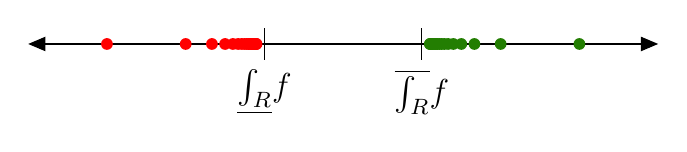
\begin{tikzpicture}
    \draw[>=triangle 45, <->] (-4,0) -- (4,0);
    \draw (-1,0.2) -- ++ (0,-0.4) node[font=\large, below] {$\underline{\int_R}f$};
    \draw (1,0.2) -- ++ (0,-0.4) node[font=\large, below] {$\overline{\int_R}f$};
    \foreach \x in {0.5,1,1.5,...,10} {
        \draw (-1 - 1 / \x,0) node[circle,fill,inner sep=1.5pt,color=red] {};
    }
    \foreach \x in {0.5,1,1.5,...,10} {
        \draw (1 + 1 / \x,0) node[circle,fill,inner sep=1.5pt,color=codegreen] {};
    }
    \end{tikzpicture}
\end{center}

\begin{definition}[Integral]
Let $R$ be a rectangle. Let $f:\; R \to \R$ be a bounded function. If $\underline{\int_R}f = \overline{\int_R}f$, we say that $f$ is Darboux integrable over $R$. And we define the integral to be their common value
$$
\int_R f = \underline{\int_R}f = \overline{\int_R}f
$$
\end{definition}


\subsection{Remarks}

\begin{theorem}[$\varepsilon$ criterion for integrability]
Let $R$ be a rectangle. Let $f:\; R \to \R$ be a bounded function.
$$
\text{$f$ is integrable over $R$} \iff \forall \varepsilon > 0,\; \exists \text{ partition $P$},\; U_P f - L_P f < \varepsilon
$$
\end{theorem}


\section{Double Integral Over Rectangles}

\subsection{Definition}

\begin{definition}[Double integral as a double Riemann sum]
The double integral of $f$ over the rectangle $R$ is
$$
\iint_R f(x,y) dA = \lim_{m,n \to \infty} \sum_{i=1}^m \sum_{j=1}^n f(x_{ij}^*, y_{ij}^*) \Delta A
$$
if the limit exists. We say the function $f$ is integrable if this limit exists.
\end{definition}

\subsection{Geometric Meaning}
If $f(x,y) \geq 0$, then the volume $V$ of the solid that lies above the rectangle $R$ and below the surface $z=f(x,y)$ is
$$
V = \iint_R f(x,y) dA
$$

\begin{figure}[h]
    \centering
    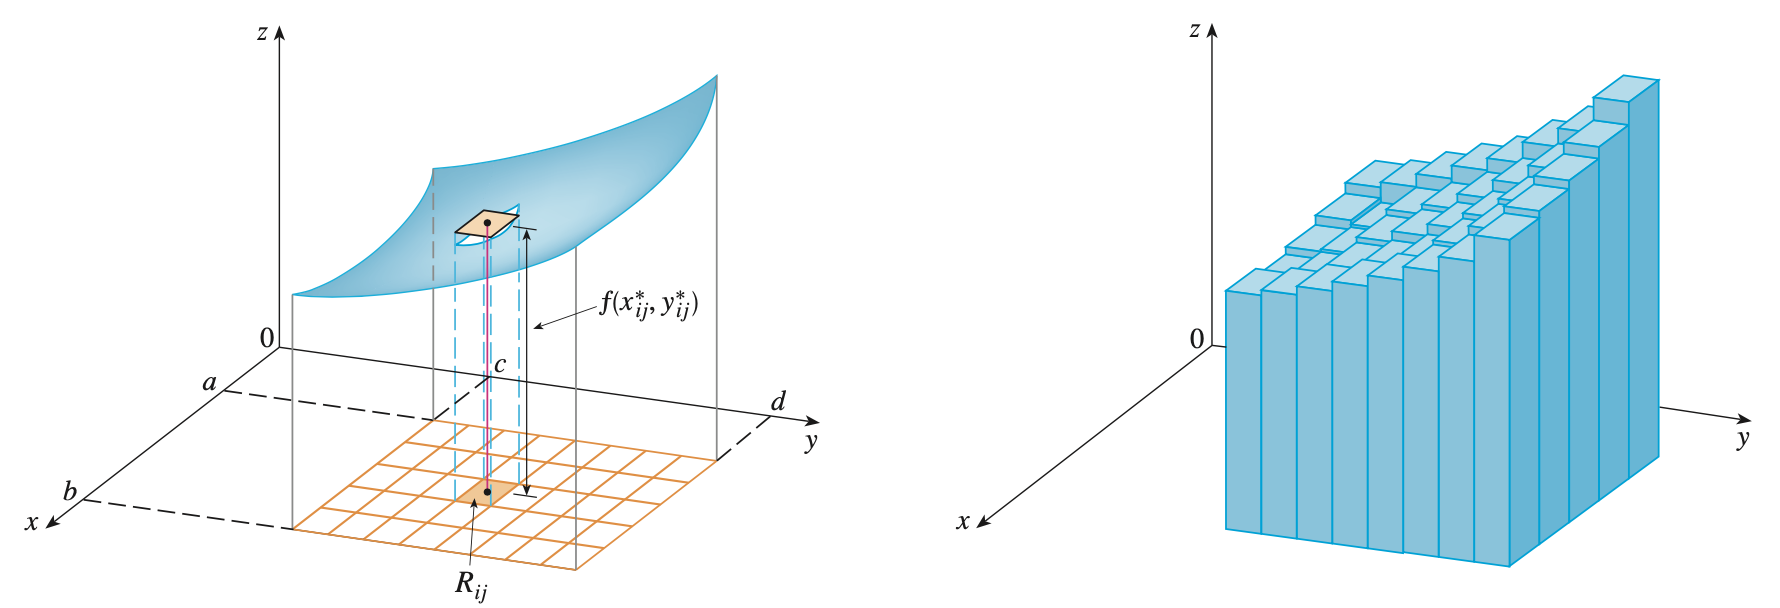
\includegraphics[width=0.6\linewidth]{figures/double-Riemann.png}
    \caption{The volume under the surface}
    \label{fig:geometric_doubleInt}
\end{figure}

\subsection{Iterated Integral}

We can evaluate a double integral over a rectangle using a method known as iterated integrals. Suppose we have a Riemann integrable function $f:\; \R^2 \to \R$ and we want to integrate it over the rectangle $R=[a,b]\times[c,d]$. We first calculate the area of the slice by integrating it with respect to $y$. This is called the partial integral with respect to $y$.
$$
A(x) = \int_c^d f(x,y) dy
$$
Then, to get the volume, we integrate $A(x)$ with respect to $x$.
$$
V = \int_a^b A(x) dx = \int_a^b\int_c^d f(x,y) dy dx
$$

Similar to the Clairaut's Theorem for mixed partial derivative, there is a theorem stating that interated integral is also symmetric.

\begin{theorem}[Fubini's Theorem]
If $f$ is continuous on the rectangle $R = \{(x,y) \mid a \leq x \leq b,\, c \leq y \leq b$ \}, then
$$
\iint_R f(x,y) dA = \int_a^b \int_c^d f(x,y) dy dx = \int_c^d \int_a^b f(x,y) dx dy
$$
\end{theorem}

\section{Double Integral Over Non-rectangles}
\subsection{Defining the Region of Integration}

It is a little bit trickier to compute a double integral over a general region. Instead of using constants when defining limits of integration, the limit of integration for one variable may be a function of the other variable.

Generally, there are two types of non-rectangular regions
$$
D = \left\{(x,y)\in \R^2 : a\le x \le b, \phi(x) \le y \le \psi(x)\right\}
$$
\begin{figure}[h]
    \centering
    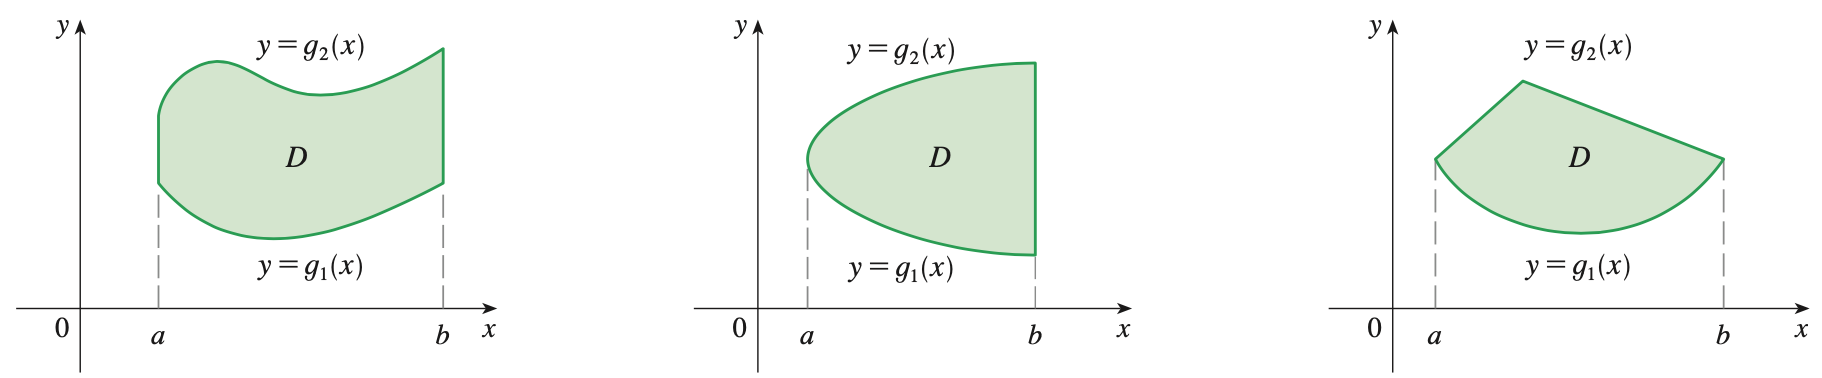
\includegraphics[width=\linewidth]{figures/type1-gen-region.png}
\end{figure}

and

$$
D = \left\{(x,y)\in \R^2 : c\le y \le d, \phi(y) \le x \le \psi(y)\right\}
$$
\begin{figure}[h]
    \centering
    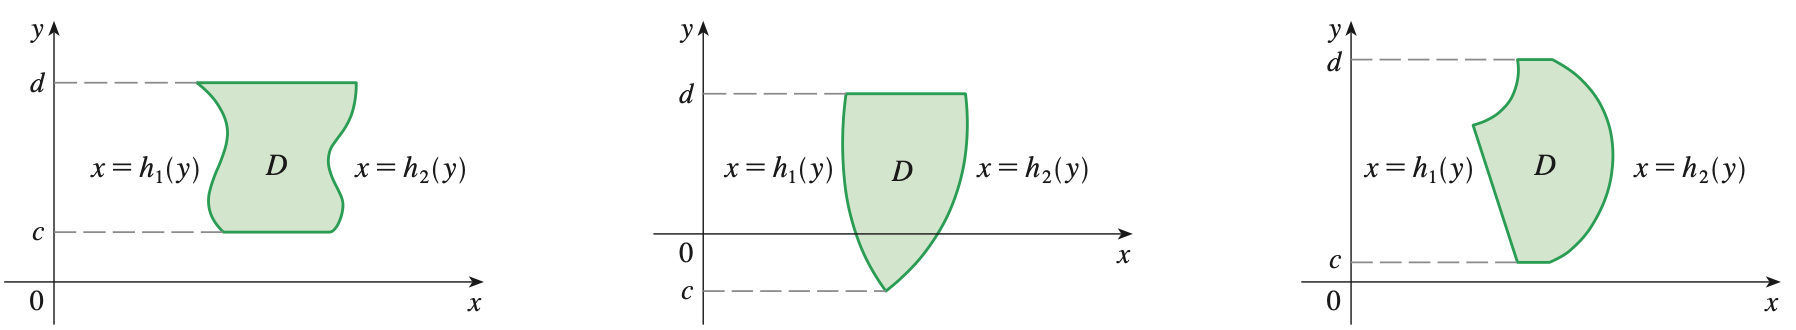
\includegraphics[width=\linewidth]{figures/type2-gen-region.png}
\end{figure}

Then, the double integral over such regions can be written as either
$$
\iint_D f\, dA =  \int_a^b \left( \int_{\phi(x)}^{\psi(x)} f(x,y) dy\right)dx
$$
or
$$
\iint_D f\, dA =  \int_a^b  \left( \int_{\phi(y)}^{\psi(y)}  f(x,y) dx\right)dy
$$

\subsection{Changing the Order of Integration}

Fubini's Theorem allows us to swap the order of integration when evaluating double integrals.

\begin{example}
Swap the order of integration for $\int_0^1 \int_x^1 \sin(y^2)dy\, dx$.

From the limits of integration, we know the region of integration is
$$
D = \{ (x,y) \mid 0 \leq x \leq 1,\, x \leq y \leq 1 \}
$$
which can also be equivalently expressed as
$$
D = \{ (x,y) \mid 0 \leq y \leq 1,\, 0 \leq x \leq y \}
$$
Hence, the integral can be rewrite as
$$
\int_0^1 \int_0^y \sin(y^2) dx\, dy
$$
\end{example}

\subsection{Combining Regions of Integration}
If $D = D_1 \cup D_2$ where $D_1$ and $D_2$ do not overlap except maybe on their boundaries, then
$$
\iint_D f(x,y) dA = \iint_{D_1} f(x,y) dA + \iint_{D_2} f(x,y) dA
$$
Using this properties, we can integrate over regions that are neither Type I or II.
\begin{figure}[h]
    \centering
    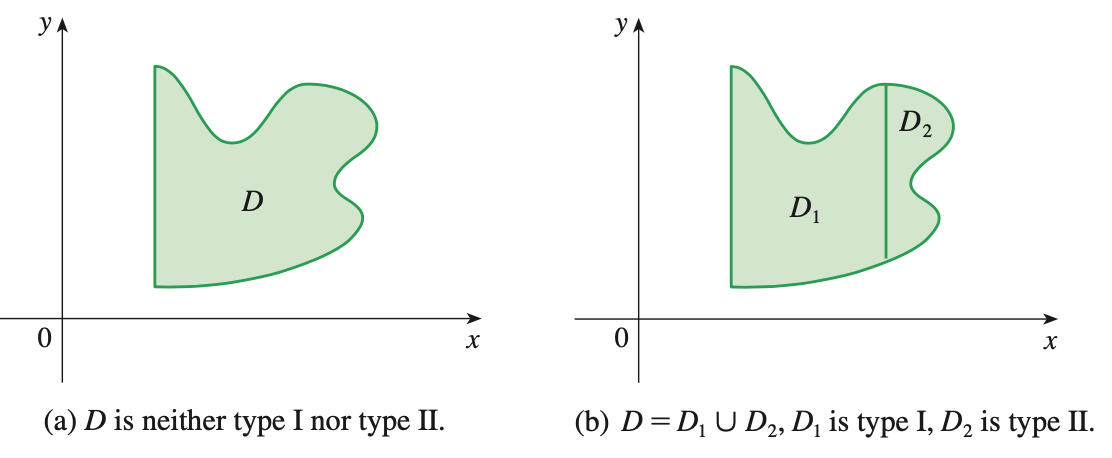
\includegraphics[width=0.7\linewidth]{figures/combine-region.png}
    \caption{Combining regions of integration}
    \label{fig:combine_regions}
\end{figure}

\section{Change of Variable}

\begin{theorem}[Change of Variable Theorem]
$$
\int_T f(\vv u) d\vv u = \int_{\vv G^{-1}(T)} f(\vv G(x)) |\det D\vv G(\vv x)|\, d\vv x
$$
\end{theorem}

\section{Double Integral in Polar Coordinates}

\section{Applications of Double Integral}

\chapter{Vector Calculus}

\section{Vector Fields}
Vector field is a function whose domain is a set of points in $\R^n$ and whose range is a set of vectors in $V_n$. In other words, a vector field assigns to each point in $\R^n$ a vector.

\begin{definition}[Vector fields]
Let $S$ be a subset of $\R^n$. A vector field in $\R^n$ is a function $\vv F:\; S \to \R^n$.
\end{definition}

Vector fields are often used in physics. Some examples include gravitational field and electric field.

\begin{example}[Gravitational fields and electric fields]
\hfill \\
Gravitational field:
$$
\vv{F}(\vv x) = - \frac{mMG}{\norm{\vv x}^3}\vv x
$$
Electric field:
$$
\vv{E}(\vv x) = \frac{\varepsilon Q}{\norm{\vv x}^3}\vv x
$$
\end{example}

\section{Graident, Divergence, and Curl}

\subsection{Definitions}

\begin{definition}[Gradient]
Let $f(x,y,z)$ be differentiable at each point in certain region of space. Then the gradient of $f(x,y,z)$, written $\nabla f$, is defined by
$$
\nabla f = \left( \partialderiv{}{x}\vv i + \partialderiv{}{y}\vv j + \partialderiv{}{z}\vv k \right) f = \left( \partialderiv{f}{x}, \partialderiv{f}{y}, \partialderiv{f}{z} \right)
$$
\end{definition}

\begin{definition}[Divergence]
Let $\vv F (x,y,z) = (P(x,y,z), Q(x,y,z), R(x,y,z))$ be defined and differentiable at each point in certain region of space (i.e. $\vv F$ defines a differentiable vector field). Then the divergence of $\vv F$, written $\nabla \cdot \vv F$, or $\mathrm{div} \vv F$ is defined by
$$
\nabla \cdot \vv F = \left( \partialderiv{}{x}\vv i + \partialderiv{}{y}\vv j + \partialderiv{}{z}\vv k \right) \cdot (P,Q,R) = \partialderiv{P}{x} + \partialderiv{Q}{y} + \partialderiv{R}{z}
$$
The divergence of a vector field is a scalar field.
\end{definition}

\begin{definition}[Curl]
If $\vv F (x,y,z) = (P(x,y,z), Q(x,y,z), R(x,y,z))$ is a differentiable vector space. Then the curl of $\vv F$, written $\nabla \times \vv F$, or $\mathrm{curl} \vv F$ is defined by
$$
\nabla \times \vv F = \left( \partialderiv{}{x}\vv i + \partialderiv{}{y}\vv j + \partialderiv{}{z}\vv k \right) \times (P,Q,R)
$$
The curl can be represented in determinant notation as
$$
\nabla \times \vv F = \begin{vmatrix}
\vv i & \vv j & \vv k \\
\partialderiv{}{x} & \partialderiv{}{y} & \partialderiv{}{z} \\
P & Q & R
\end{vmatrix} = \left(\partialderiv{R}{y}-\partialderiv{Q}{z},\, \partialderiv{P}{z}-\partialderiv{R}{z},\, \partialderiv{Q}{x}-\partialderiv{P}{y} \right)
$$
The curl of a vector field defines a vector field.
\end{definition}

\subsection{Geometric Interpretation}
Geometrically, given a point, the divergence tells us whether a particle at that point tends to diverge or converge, and by how much. More technically, the divergence represents the volume density of the outward flux of a vector field from an infinitesimal volume around a given point. When $\Div \vv F = 0$, then $\vv F$ is said to be \textit{incompressible}.

\begin{figure}[h]
    \centering
    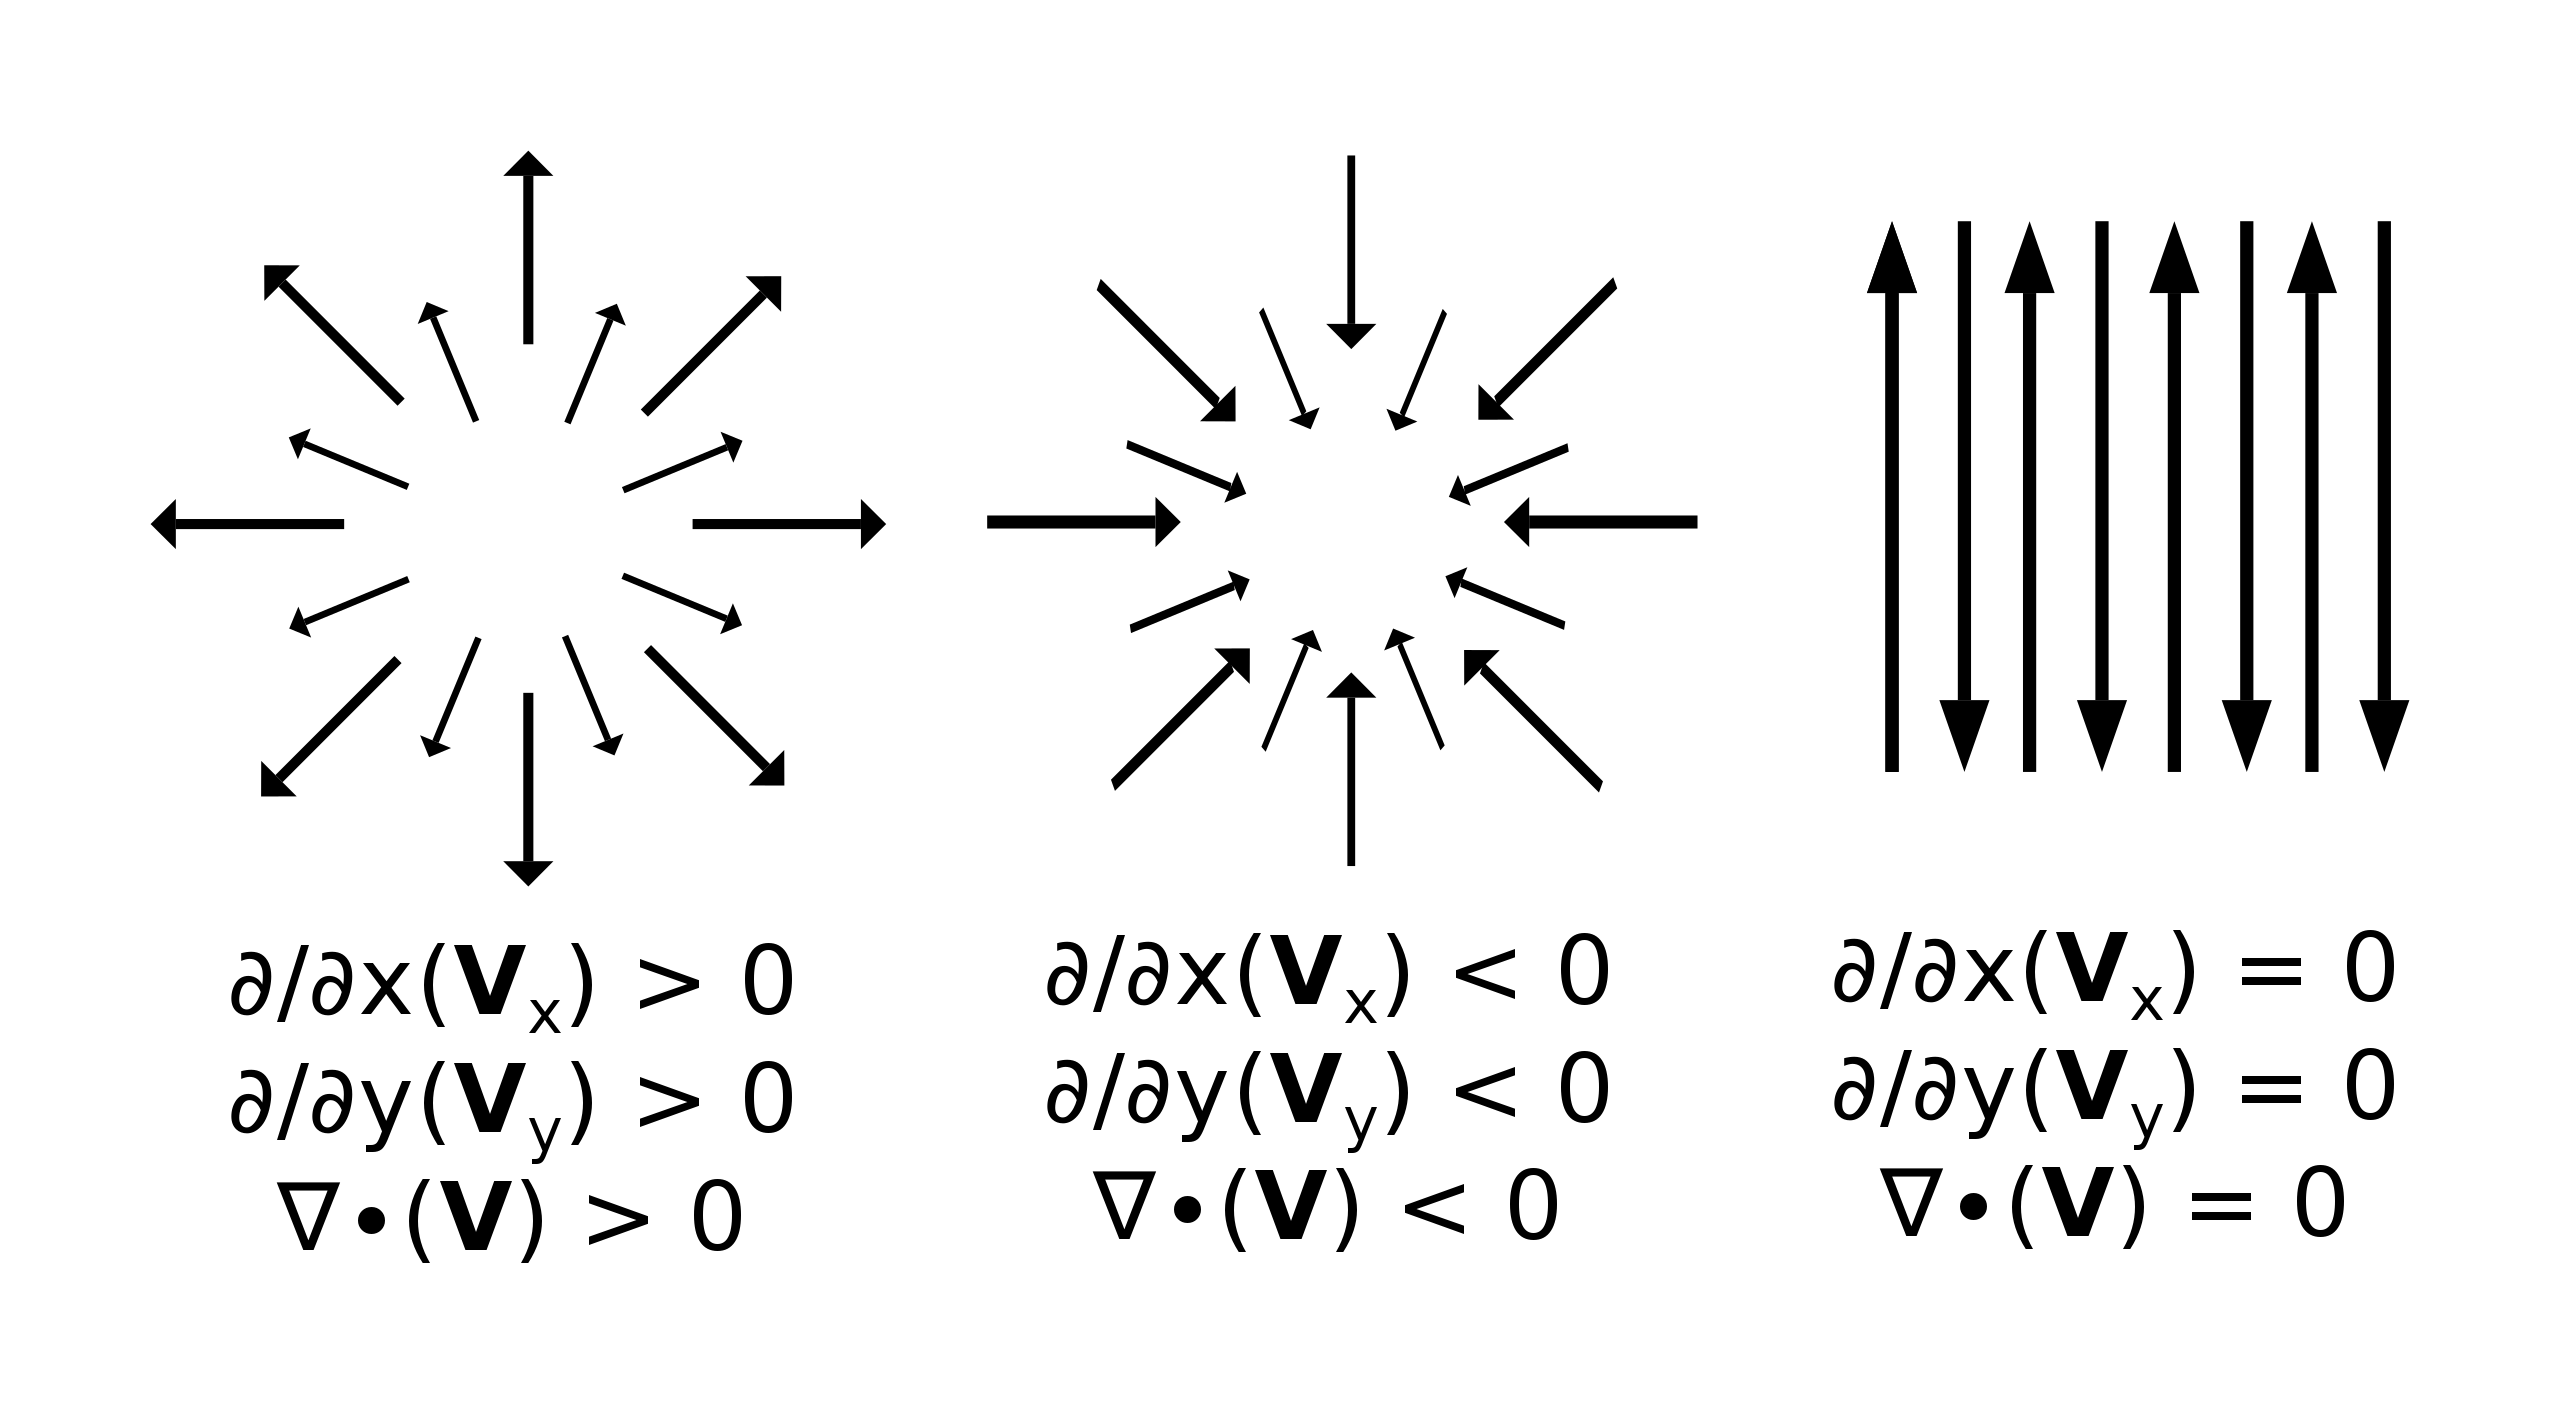
\includegraphics[width=0.5\linewidth]{figures/divergence.png}
    \caption{A positive divergence indicates that particles tend to diverge away from that point; a negative divergence indicates that particles tend to converge at that point; a zero divergence means that there is no net density change at that point.}
    \label{fig:divergence}
\end{figure}

Curl is geometrically associated with rotation of particles in a vector field. Curl tells us the direction of rotation at a given point. To determine the direction of the curl, we use the right-hand rule just like when we are determining the angular momentum of a rotating object. Imagine curling your right hand around the direction of rotation and stick up your thumb, your thumb should point in the direction of the curl.

\begin{figure}[h]
    \centering
    \raisebox{-0.5\height}{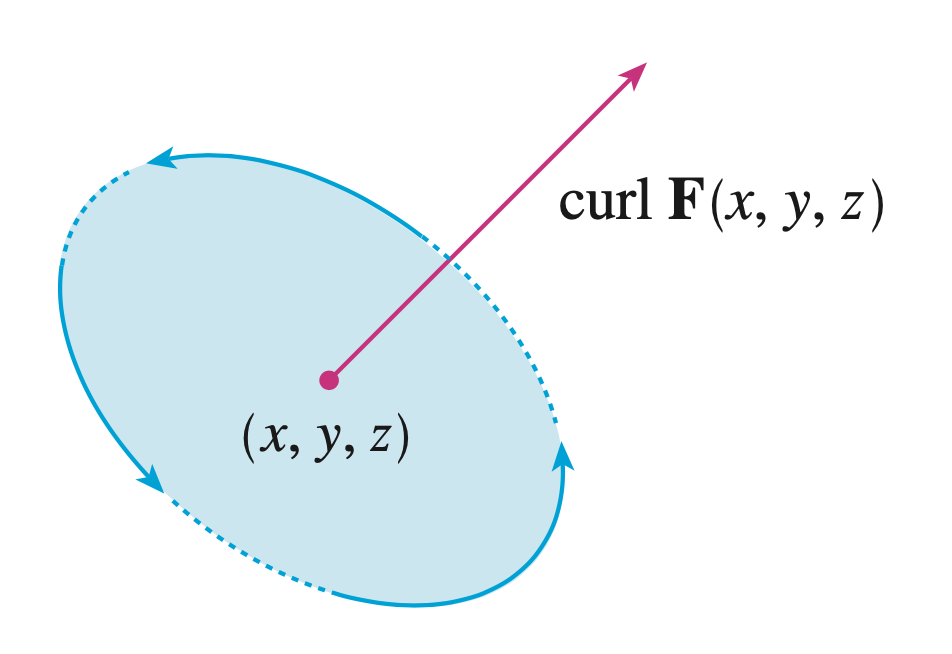
\includegraphics[width=0.25\linewidth]{figures/curl-simple.png}}
    \qquad
    \raisebox{-0.5\height}{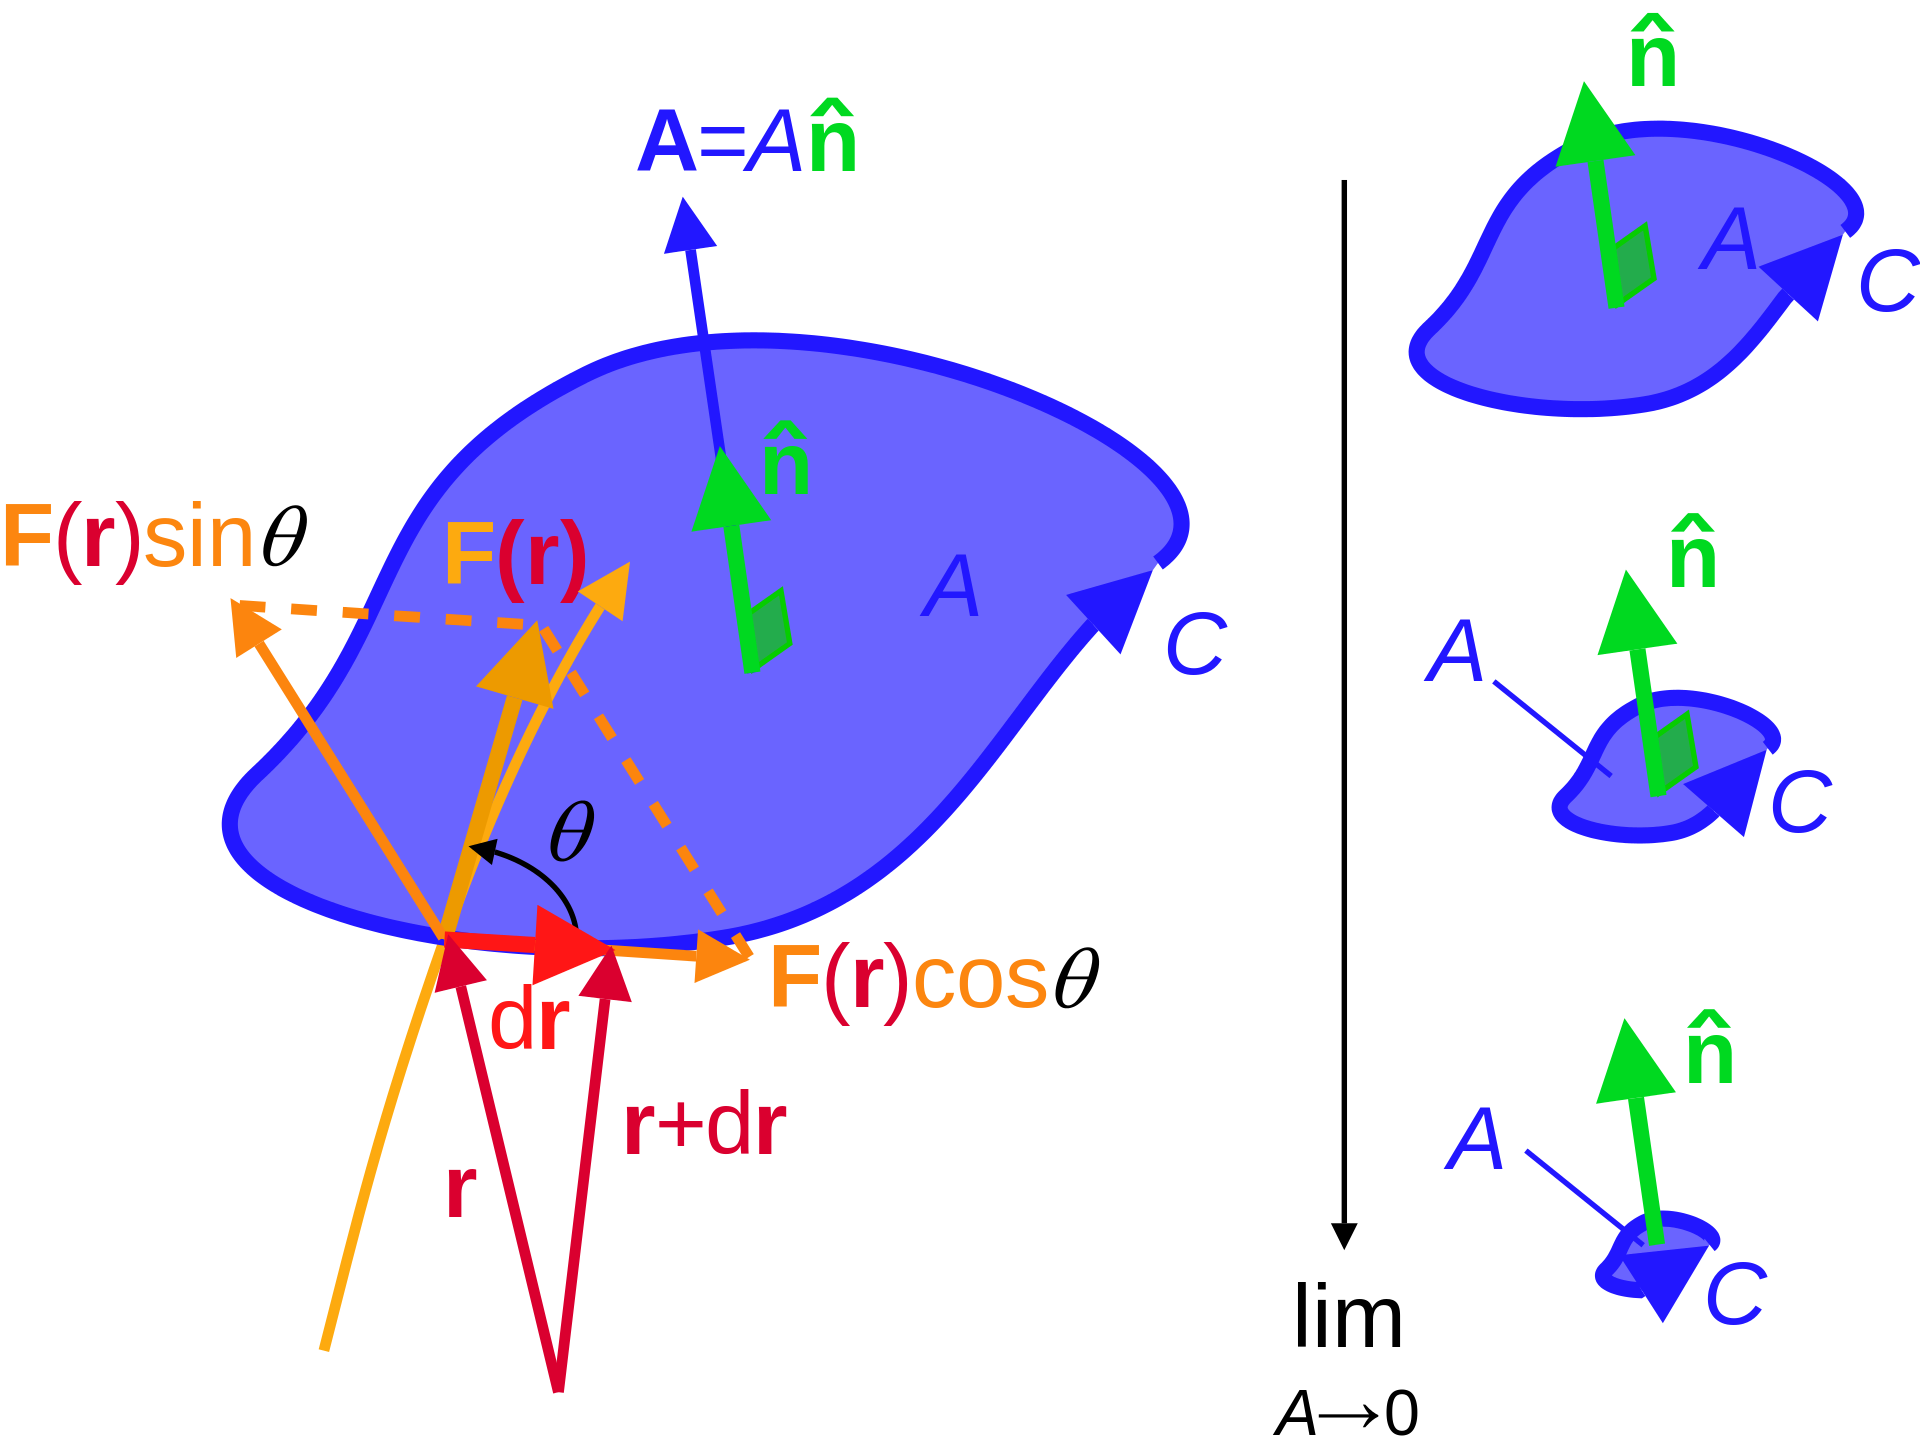
\includegraphics[width=0.4\linewidth]{figures/curl-limit.png}}
    \qquad
    \raisebox{-0.5\height}{
\includegraphics[width=0.2\linewidth]{figures/curl-righthand.png}}
    \caption{From left to right: simple diagram showing relationship between curl and vector field; curl as a limit; the right-hand rule for determining particle rotation.}
    \label{fig:curl}
\end{figure}

\subsection{Properties}
There are some properties involving grad, div, and curl

\begin{theorem}[Sum rules]
$$
\begin{aligned}
\Grad(f+g) &= \Grad(f) + \Grad(g) \\
\Div(\vv F + \vv G) &= \Div(\vv F) + \Div(\vv G) \\
\Curl(\vv F + \vv G) &= \Curl(\vv F) + \Curl(\vv G) \\
\end{aligned}
$$
\end{theorem}

\begin{theorem}[Product rules]
$$
\begin{aligned}
\Grad (fg) &= f \Grad g + g \Grad f  \\
\Div (f\vv G) &= f\Div \vv G + (\Grad f) \cdot \vv G   \\
\Curl (f\vv G) &= f \Curl \vv G +(\Grad f) \times \vv G \\
\Div(\vv F\times \vv G)&= \vv G\cdot \Curl \vv F - \vv F\cdot \Curl \vv G\\
\Curl(\vv F\times \vv G)&=
(\vv G\cdot \nabla)\vv F + (\Div \vv G)\vv F+
(\vv F\cdot \nabla)\vv G + (\Div  \vv F) \vv G \\
\Grad(\vv F\cdot \vv G) &=
(\vv G\cdot \nabla)\vv F + \vv G\times \Curl \vv F -
(\vv F\cdot \nabla)\vv G - \vv F\times \Curl \vv G 
\end{aligned}
$$
where
$$
(\vv F\cdot \nabla)\vv G = \sum_{j=1}^3 F_j \partial_j \vv G,
\qquad 
(\vv G\cdot \nabla)\vv F = \sum_{j=1}^3 G_j \partial_j \vv F.
$$
\end{theorem}

\begin{definition}[Laplacian]
For a twice-differentiable function $f:\; \R^n \to \R$, the Laplacian of $f$ is
$$
\Div(\Grad(f)) = \nabla \cdot (\nabla f) = \nabla^2 f = \Delta f = \sum_{j=1}^n \partial_{jj}f
$$
For $f:\; \R^3 \to \R$,
$$
\Delta f = \nabla^2 f = \frac{\partial^2 f}{\partial x^2} + \frac{\partial^2 f}{\partial y^2} + \frac{\partial^2 f}{\partial z^2}
$$
$\Div(\Grad()),\, \nabla \cdot \nabla,\, \nabla^2,\, \Delta$ are all acceptable notations for Laplacian. $\nabla^2$ is often used in mathematics, and $\Delta$ is more often used in physics.
\end{definition}

In addition, we have the following properties:

The curl of a gradient is zero.
$$
\nabla \times (\nabla \vv F) = \Curl(\Grad(\vv F)) = 0
$$

The divergence of a curl is also zero.
$$
\nabla \cdot (\nabla \times \vv F) = \Div(\Curl(\vv F)) = 0
$$

\section{Conservative Vector Fields}

The divergence and curl of a vector field can be used to understand some of the properties of vector fields. An important family of vector fields are called conservative vector fields.

\begin{definition}[Conservative vector fields]
A vector field $\vv F$ is called conservative if it is the gradient of some scalar function. That is, if there is a function $f$ such that
$$
\nabla f = \vv F = \left( \partialderiv{f}{x},\, \partialderiv{f}{y},\, \partialderiv{f}{z} \right)
$$
The function $f$ is called the potential function of $\vv F$.
\end{definition}

The are some theorems that allow us to show that a vector field is conservative.

\begin{theorem}
Let $\vv F = P\vv i + Q\vv j = (P,Q)$ be a vector field. If $\vv F$ is conservative and $P(x,y)$, $Q(x,y)$ have continuous first-order partial derivatives on a domain $D$, then throughout $D$ we have
$$
\partialderiv{P}{y} = \partialderiv{Q}{x}
$$
The converse of this theorem is not necessarily true. But given some additional constraints, it becomes true.
\end{theorem}

\begin{theorem}
Let $\vv F = P\vv i + Q\vv j = (P,Q)$ be a vector field. Let $D$ be an open simply connected region of the plane. If $P(x,y)$, $Q(x,y)$ have continuous first-order partial derivatives on $D$, and throughout $D$ we have
$$
\partialderiv{P}{y} = \partialderiv{Q}{x}
$$
Then, $\vv F$ is a conservative vector field.
\end{theorem}

\section{Line Integral}

\subsection{Line Integral of Scalar Field}

A line integral of a scalar field or of a function $f(x,y)$ is represented as
$$
\int_C f(x,y) ds
$$


\begin{definition}[Line integral]

If $f$ is defined on a smooth curve $C$ given by a parametric equation
$$
x = x(t) \qquad y = y(t) \qquad a \leq t \leq b
$$
for some $a,b \in \R$, or equivalently by the vector equation $\vv r(t)=(x(t),y(t))$, then the line integral of $f$ along $C$ is
$$
\int_C f(x,y) ds = \lim_{n\to\infty} \sum_{i=1}^n f(x_i^*, y_i^*) \Delta s_i
$$
if this limit exists.
\end{definition}

Using the arc length formula, we know that the length of $C$ is
$$
\int_a^b \sqrt{\left( \frac{dx}{dt} \right)^2 + \left( \frac{dy}{dt} \right)^2} dt
$$
Then we can rewrite the definition as
$$
\int_C f(x,y) ds = \int_a^b \left[ f(x(t),y(t)) \sqrt{\left( \frac{dx}{dt} \right)^2 + \left( \frac{dy}{dt} \right)^2} \right] dt
$$

\subsection{Line Integral of Vector Field}

\begin{definition}[Line integral of vector field]
Given a vector field $\vv F:\; S \to \R^n$, and a curve $C \subset S \subseteq \R^n$ parameterized by $\vv g$, we define the line integral of $\vv F$ over $C$ as
$$
\int_C \vv F \cdot dx = \int_a^b  \vv F(\vv g(t)) \cdot \vv{g}'(t) dt
$$
\end{definition}

\section{The Fundamental Theorem of Line Integral}

\begin{theorem}[The Fundamental Theorem of Line Integral]
Suppose that $f:\; \R^n  \to \R$ is a function of class $C^1$, and that $C$ is a curve oriented by $\vv x = \vv g(t)$ where $a \leq t \leq b$. Then, we can compute the line integral of the vector field $\vv F = \nabla f$ as follows
$$
\begin{aligned}
\int_C \nabla f \cdot d\vv x &= \int_a^b  \nabla f(\vv g(t)) \cdot \vv g'(t)dt \\
&= \int_a^b \frac{d}{dt} f(\vv g(t)) dt & \text{by Chain Rule} \\
&= f(\vv g(b)) - f(\vv g(a)) & \text{by FTC}
\end{aligned}
$$
\end{theorem}

This theorem tells us two things:
\begin{itemize}
    \item The line integral over a conservative vector field does not depend on the path. It only depends on the starting and end points. More formally, if $C_1= \vv r_1(t)\; a \leq t \leq b$ and $C_2 = \vv r_2(t) \; c \leq t \leq d$ are two continuous curves such that $r_1(a)=r_2(c)$ and $r_1(b)=r_2(d)$, that is the curves have the same initial and end points, then if $\vv F$ is a conservative vector field,
    $$
    \int_{C_1} \vv F \cdot d\vv r = \int_{C_2} \vv F \cdot d\vv r
    $$
    This property is called independence of paths.
    \item If $C$ is a continuous path with initial point $\vv r(a)$ and end point $\vv r(b)$, and we denote by $-C$ the curve starts at $\vv r(b)$ and ends at $\vv r(a)$, then for every conservative vector field $\vv F$
    $$
    \int_{-C} \vv F \cdot d\vv r = -\int_C \vv F \cdot d\vv r
    $$
    In other words, changing the orientation of $C$ only changes the sign of the line integral.
    \item For any closed curve $C$, if the vector field $\vv F$ is conservative, then
    $$
    \oint_C \vv F \cdot d\vv r = 0
    $$
\end{itemize}

\section{Green's Theorem}

\begin{definition}[Stokes' orientation]
Given a regular region with piecewise smooth boundary, we define the Stokes' orientation to be the orientation of the boundary such that the interior of the set is always on the left of the direction of travel.
\end{definition}

\begin{theorem}[Green's Theorem]
Let $C$ be a Stokes oriented, piecewise-smooth, simple closed curve in the plane and let $D$ be the region bounded by $C$. If $P(x,y)$ and $Q(x,y)$ have continuous derivatives on an open region that contains $D$ and define $\vv F=(P,Q)$, then
$$
\oint_C \vv F \cdot d\vv r = \oint_C P \, dx + Q \, dy = \iint_D \left( \partialderiv{Q}{x} - \partialderiv{P}{y} \right) dA
$$
\end{theorem}

\section{Stokes' Theorem}

\begin{theorem}[Stokes' Theorem]
Let $S$ be a Stokes oriented piecewise-smooth surface that is bounded by a simple, closed, piecewise-smooth boundary curve $\partial S$. Let $\vv F$ be a vector field whose components are $C^1$ on an open region in $\R^3$ that contains $S$. Then,
$$
\int_{\partial S} \vv F \cdot d\vv r = \iint_S \Curl \vv F \cdot d\vv S = \iint_S \Curl \vv F \cdot \hat{n}\, dA
$$
\end{theorem}




\end{document}